\section{Recommendations for Run 2 b-taggers}

\subsection{High level taggers: DL1 series}


The task of $b$-tagging is \emph{almost} as old as collider physics.
These low level algorithms characterizing the impact parameters and vertices have been around since the inception of ATLAS, and the RNN development and optimization studies were also before my time.
However, a part of taking over the maintenance of the RNN for my ATLAS qualification task, I produced the first RNNIP training that was used by the whole collaboration.

The developments that we worked together on went beyond just my own work, as the high level tagger that aggregated information from the low level is now a NN-based solution. The Run 2 recommended tagger is the DL1r algorithm, which includes inputs from the Low-Level taggers described in \Sect{\ref{sec:low-level}}, with the inputs summarized below:


We combine the low level taggers into a high-level one, the DL1r algorithm, combining information from the low-level taggers:
\begin{itemize}%[noitemsep]
	\item The jet \pt and $\eta$ (to learn about the correlations between the jet's energy with the low-level tagger decisions
	\item \textbf{IP2D and IP3D}: Since the Neyman Pearson lemma says that the optimal discriminator between two probability distributions is the ratio of probabilities, we pass the $\log p_b / p_c$, $\log p_b / p_l$, and $\log p_c / p_l$ as DL1r NN inputs (2 IP taggers x 3 inputs = 6 inputs) 
	\item \textbf{RNNIP}: For this round of recommendations, we have a two step tagger training process. I first optimized the hyperparameters of the RNN and then the DL1r algrothm accepted as inputs the outputs RNNIP outputs: $p_b$, $p_c$, and $p_l$ (3 inputs)
	\item \textbf{SV1}: vertex information (variables in \Tab{\ref{tab:sv1-inputs}}) (8 inputs)
	\item \textbf{JF}: displaced vertices characteristics, \Tab{\ref{tab:jf-inputs}} (20 inputs).
\end{itemize} 

For the low-level algorithms, sometimes the algorithms don't always ``succeed'' or have a non-trivial output (i.e, no tracks were selected by the tight selection cuts of the IPXD algorithms, or the vertex fit failed to find a secondary vertex). To let the NN know that these are cases where the low-level algorithm is just passing a default value, a boolean variable is passed if this algorithm has default values. This adds an additional 5 inputs: \texttt{IP2D\_isDefault}, \texttt{IP3D\_isDefault}, \texttt{SV1\_isDefault}, \texttt{JF\_isDefault}, and \texttt{JFc\_isDefualt} (since the \Pqc-tagging variables are only calculated when JF finds exactly one SV. 
For the DL1r training, the default values are set to the mean of the distribution (to be uninformative for the NN discrimination), except for variables where it makes physical sense to set it to 0 for no SV being found (such as the mass or the energy of the SV is set to 0 if no SV is found).
This makes the total \# of input variables:

\begin{center}
\# DL1r inputs = 2 \small{(jet \pt, $\eta$)} + 6 (IPXD) + 3 (RNNIP) + 8 (SV1) + 20 (JF) + 5 (boolean defaults) = 44
\end{center}

As is common in ML applications, these inputs are then pre-processed to have zero mean and unit variance (except for the boolean default indication variables).

The architecture used was optimized in a grid search and has 8 hidden layers with 256, 128, 60, 48, 36, 24, 12, and 6 hidden nodes per layer, with ReLU non-linearities. A softmax output layer with 3 output nodes for the \Pqb, \Pqc, and light jets. The categorical cross entropy loss is used, and the parameters of the NN are optimized with a stochastic gradient descent optimizer adam \cite{adam} with a learning rate of 0.01, and a batch size of 15,000 jets.

As mentioned in the RNNIP section, we don't want to make classification decisions just based on the input training kinematics.
Although for the RNNIP training, we ameliorated this dependence by reweighting the \Pqb and \Pqc-jet \pt distributions to match the light jet distribution, the DL1r training setup uses (what I believe is) a better paradigm of resampling the input jets.

The input training sample discretizes the jets in the (\pt, $\eta$) plane, and then samples from the jet flavor distributions to have a uniform number of events across the  (\pt, $\eta$) spectrum and across the jet flavors.
In this procedure - 22~million jets are used for the input training for DL1r, with an equal proportion of $b$, $c$, and light jets.

The comparisons of the DL1r tagger is made against two other taggers: DL1r, which uses the same inputs as DL1r -- except for the RNNIP variables -- and MV2, which uses the same inputs as DL1, but is a BDT-based tagger instead of a NN based one.


\hl{Insert smth about how DL1 is more space efficient than MV2}


\subsection{Evaluating tagger performance}

\textbf{I might want to put this in the RNNIP section though -- depending on if I show any roc curves there or not.}

The class probabilities predicted by the model outputs ($p_b$, $p_c$, and $p_l$), are combined into a $b$-tagging discriminant:
\begin{equation}
 D_b = \log \frac{p_b}{(1-f_c) p_l + f_c p_c}
 \label{eq:dipsdiscriminant}
\end{equation}
where $f_c$ is a free parameter that balances between the rejection of light-flavour vs $c$-jets for a given efficiency of selecting $b$-jets, and can be optimized post-training. 
A value of $f_c = 0.07$ was used in these studies  as this is representative of the fraction of $c$-jets relative to non $b$-jets in $t\bar{t}$ events. 


\subsection{PFlow optimization}

\textbf{Hybrid sample definition}

In the course of the completion of this thesis, the collaboration switched from using EMTopo jets (which reconstruct a jet from the topo clusters in the calorimeter) to  using PFlow jets which cluster a jet using particle flow candidates that takes into account the better resolution of the tracker for reconstructing lower momentum objects. This improves the jet reconstruction algorithm in two ways. (1) We gain a better reconstruction of the jet \pt resolution (shown by 

\begin{itemize}
	\item Switching from EMTopo to PFlow
	\item Main improvement that we expected for $b$-tagging would be better with the better angular resolution for the jet axis
\end{itemize}

\begin{figure}[htbp]
  \centering
  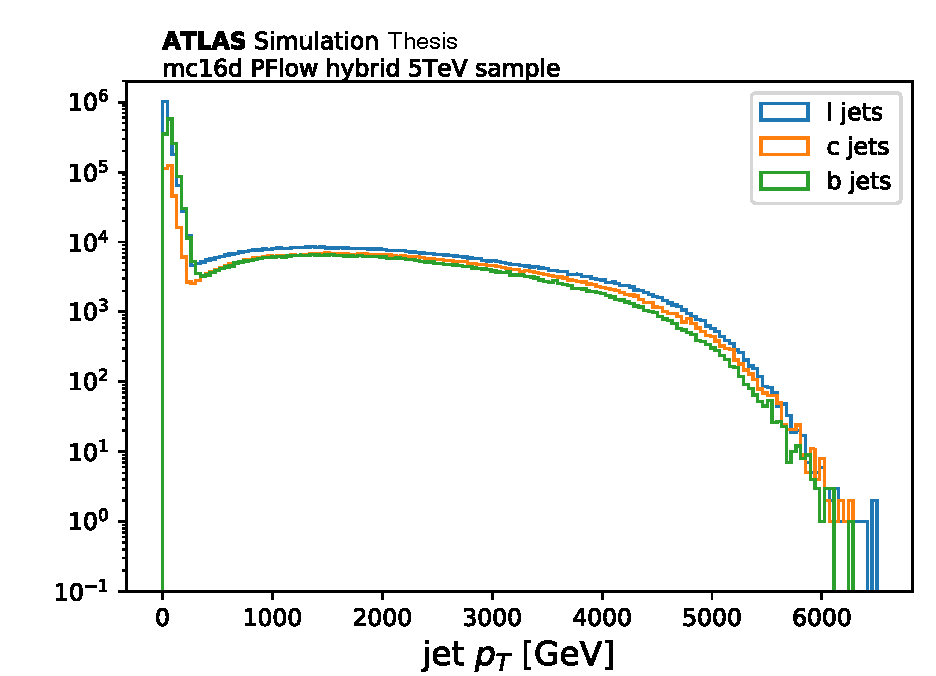
\includegraphics[width=.6\textwidth]{figures/ftag/PFlow trainings/pflow-pt-extended-hybrid}
  \caption{The \pt spectrum for training the Full Run 2 FTAG recommendations.}
  \label{fig:pflow-pt-extended-hybrid}
\end{figure}



\textbf{RNNIP optimization}

An illustration of why the task of \Pqb-tagging becomes harder at high \pt is illustrated in \Fig{\ref{fig:hf-ftag-tracks}}.


\begin{figure}[htbp]
  \centering
  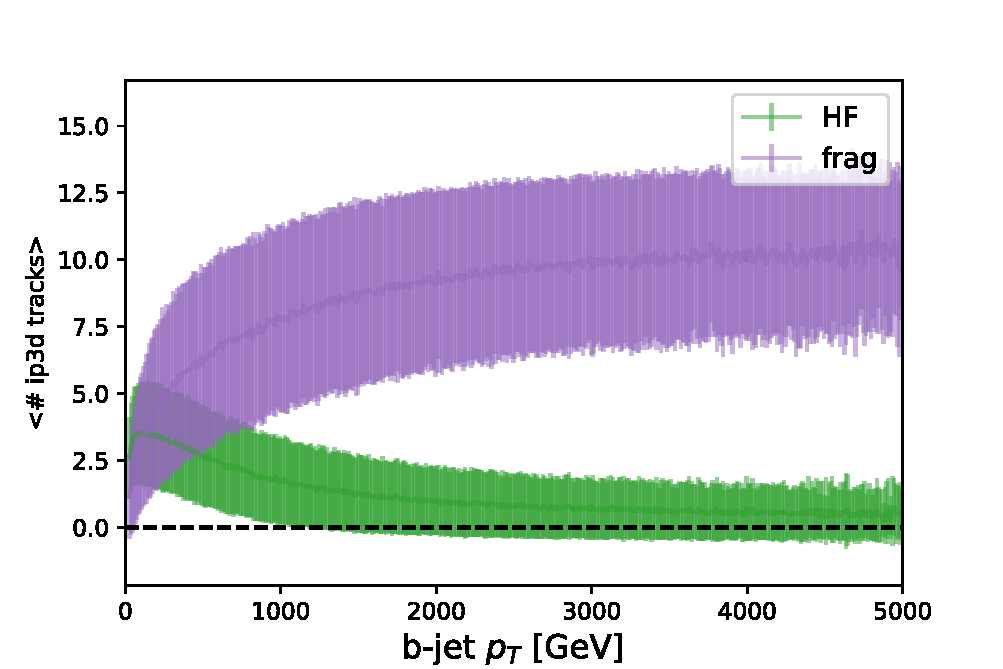
\includegraphics[width=.6\textwidth]{figures/ftag/PFlow trainings/hf-frag-tracks}
  \caption{The evolution of heavy flavor compared to the number of fragmentation tracks that have $\pt > 1~\mathrm{GeV}$, $|d_0| < 1$~mm, $|z_0 \sin \theta < 1.5$~mm, .}
  \label{fig:hf-frag-tracks}
\end{figure}


Our optimization for the RNNIP training for the PFlow tagger uses 400 hidden units in the \ldots LSTM cell.
This is an increase from the 50 hidden units of \cite{ATL-PHYS-PUB-2017-003} since training over the much larger dynamic range needed a more complex architecture.
\textbf{Do I remember what lr I used?}
The training was done with the adam optimizer, using 5 million jets, and 20\% of the dataset was held out as a validation set, and the training was stopped when the validation loss had not improved in the last 20 epochs.


\begin{figure}
\centering
\subfloat[light rejection]{
	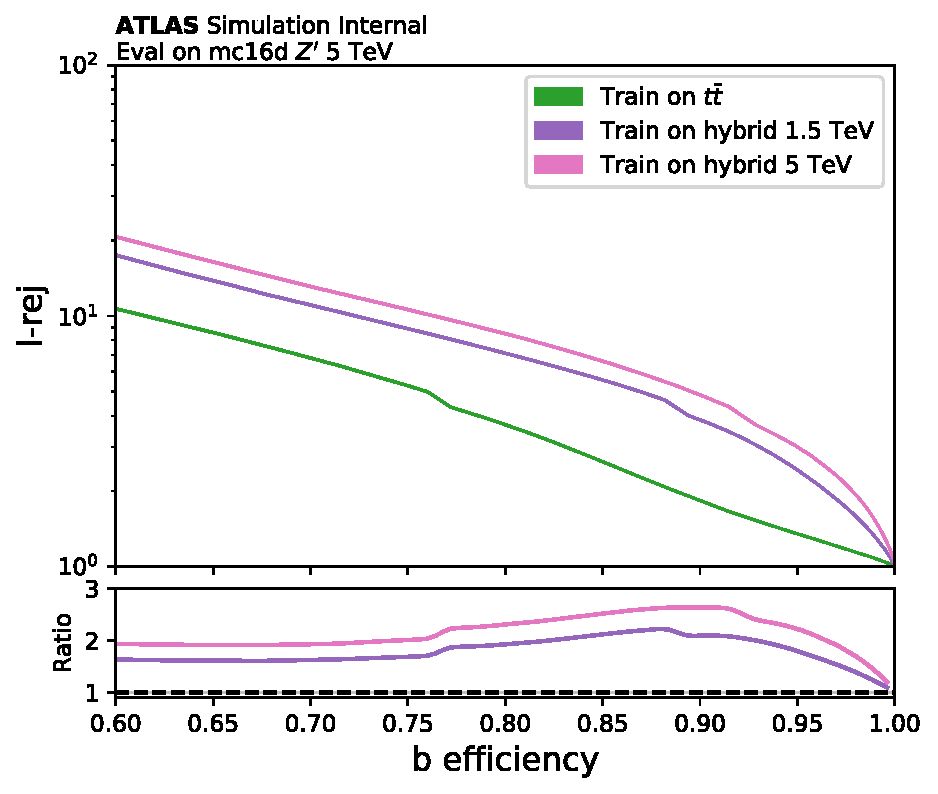
\includegraphics[width=0.45\textwidth]{{figures/ftag/PFlow\ Trainings/Zprime-l-roc}}
	}
\subfloat[\Pqc rejection]{
	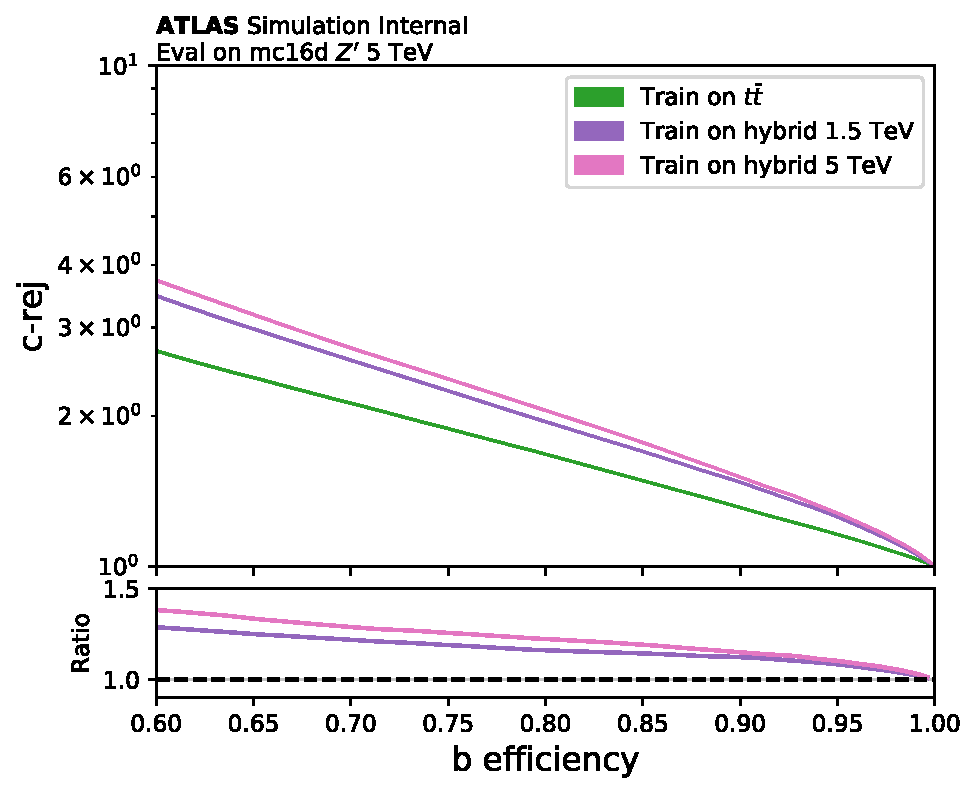
\includegraphics[width=0.45\textwidth]{{figures/ftag/PFlow\ Trainings/Zprime-c-roc}}
	}
\caption{}
\label{fig:Zprime-c-roc}
\end{figure}


\begin{figure}
\centering
\subfloat[light rejection]{
	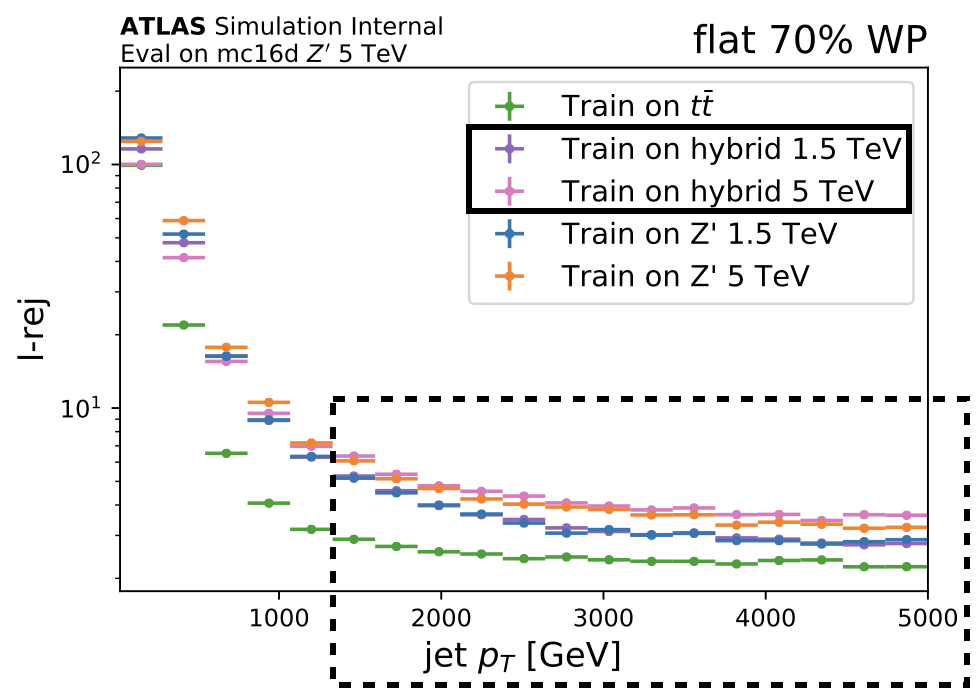
\includegraphics[width=0.45\textwidth]{{figures/ftag/PFlow\ Trainings/Zprime-l-pt}}
	}
\subfloat[\Pqc rejection]{
	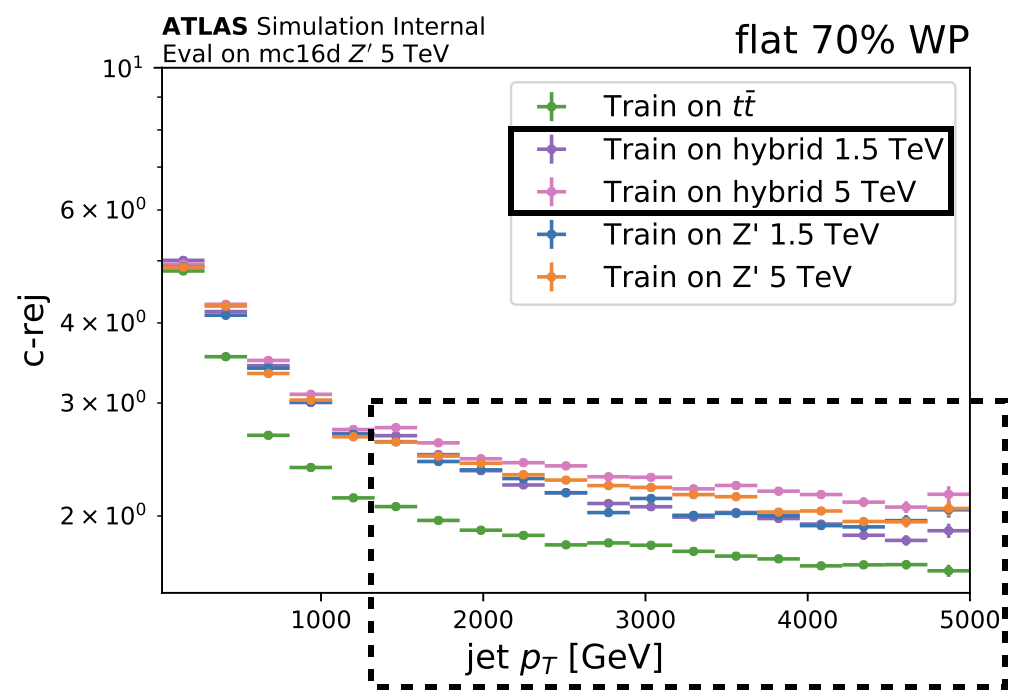
\includegraphics[width=0.45\textwidth]{{figures/ftag/PFlow\ Trainings/Zprime-c-pt}}
	}
\caption{}
\label{fig:Zprime-pt}
\end{figure}



\begin{figure}
\centering
\subfloat[light rejection]{
	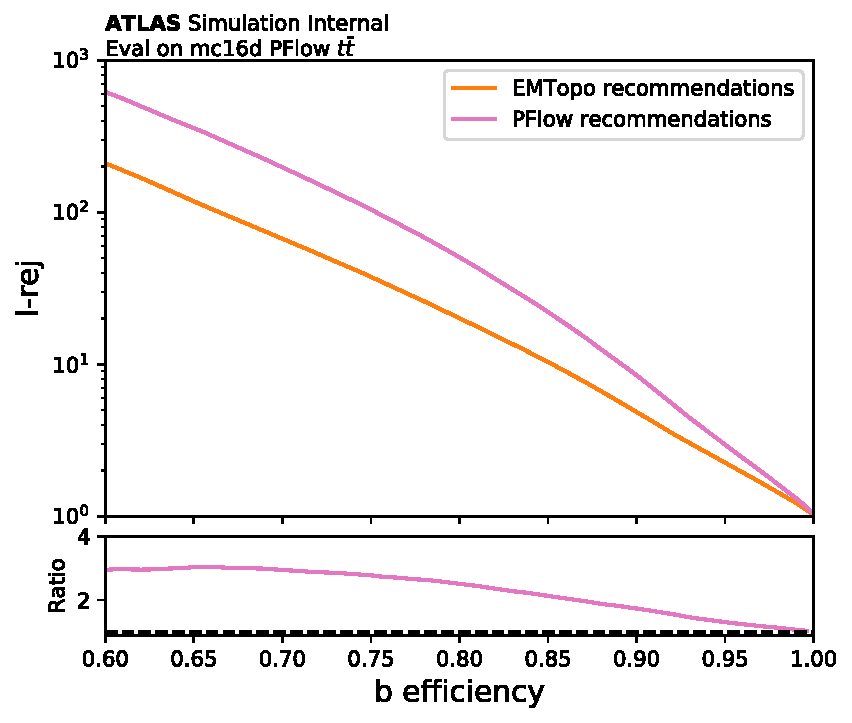
\includegraphics[width=0.45\textwidth]{{figures/ftag/PFlow\ Trainings/topo-vs-pflow-l-rej}}
	}
\subfloat[\Pqc rejection]{
	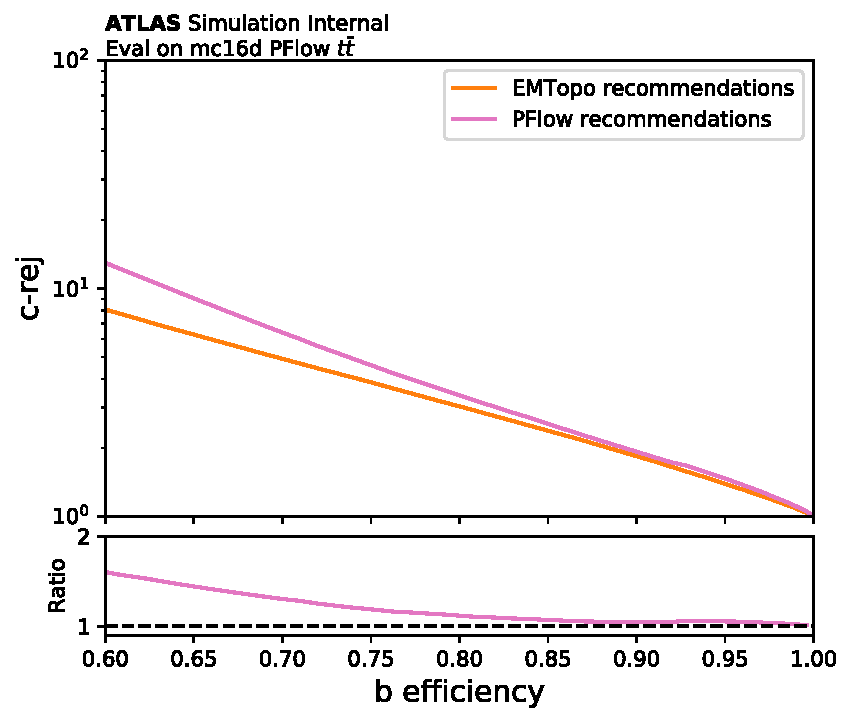
\includegraphics[width=0.45\textwidth]{{figures/ftag/PFlow\ Trainings/topo-vs-pflow-c-rej}}
	}
\caption{}
\label{fig:topo-pflow}
\end{figure}

The EMTopo training recommendation was from the 2017 retraining campaign:

Rafael showed we see retraining gains due to the kinematics changes with hdamp from mc15 -> mc16

Dedicated retraining on new pflow jet collection

Plus the RNN improvements from this year


An illustration of how this newly retrained RNN compares to some other low level taggers is shown in \Fig{\ref{fig:rnnip-cf-sv1-jf}}.

\begin{figure}
\centering
	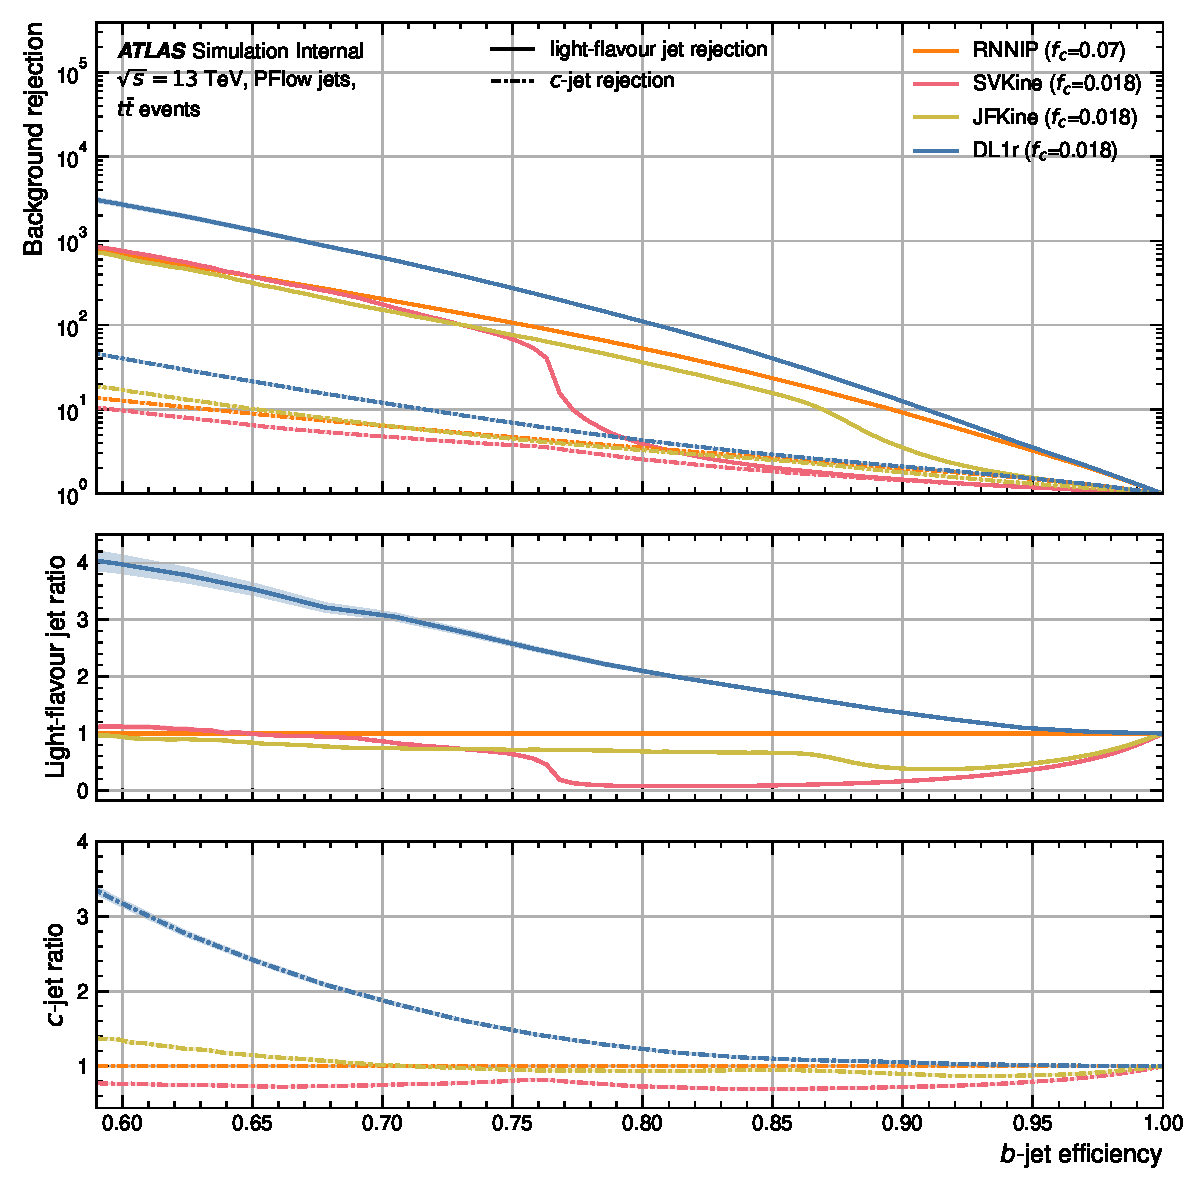
\includegraphics[width=0.7\textwidth]{{figures/ftag/PFlow\ Trainings/roc_rnnip_kine_DL1r_ttbar}}
	\caption{Comparision of the performance of the low level taggers \cite{ANA-FTAG-2019-07}}
\label{fig:rnnip-cf-sv1-jf}
\end{figure}


\textbf{DL1r results}


% PFlow results link
% http://atlas.web.cern.ch/Atlas/GROUPS/PHYSICS/PLOTS/FTAG-2019-005/
\def\jetdef{PFlow}
\def\figpath{figures/ftag/\jetdef \ trainings}

\begin{figure}[htbp]
    \centering
    % light
    \subfloat[]{ 
            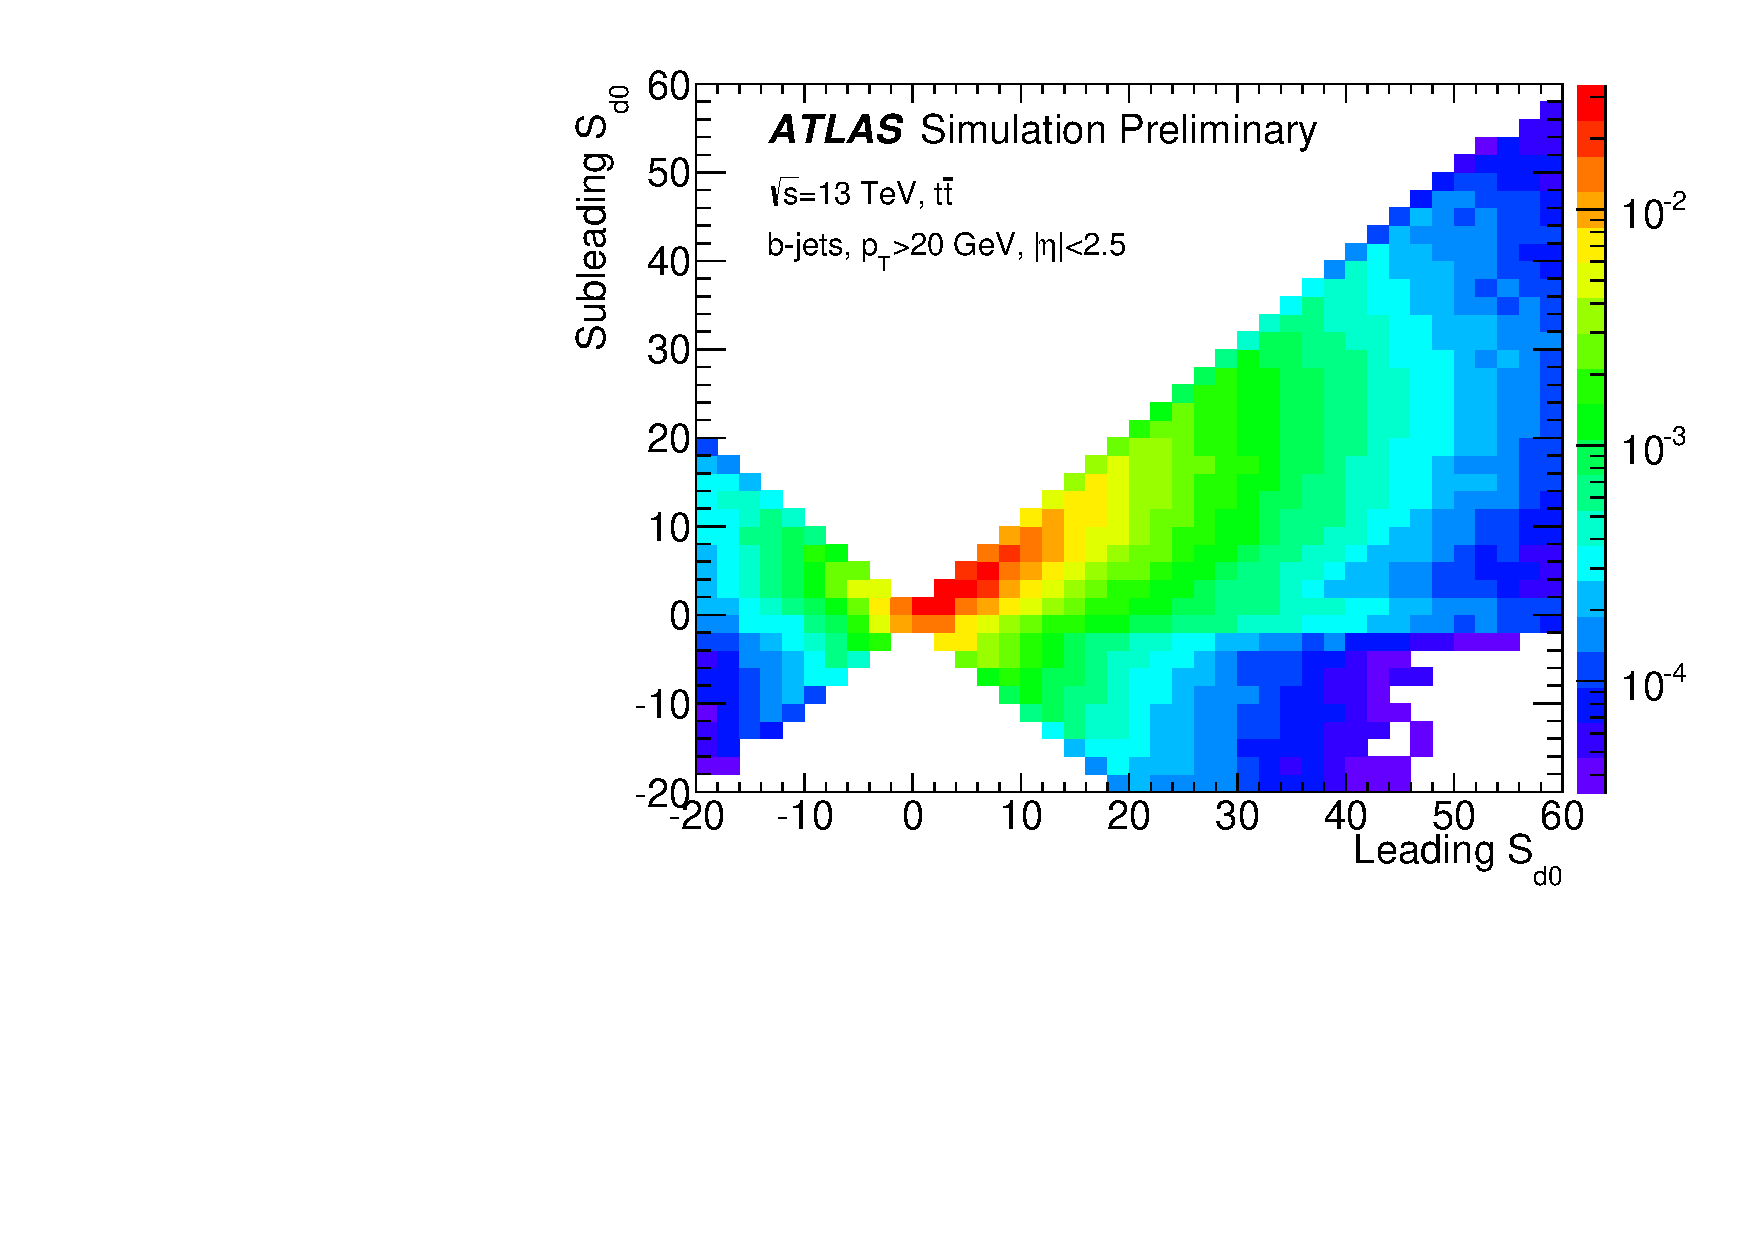
\includegraphics[width=0.48\linewidth]{\figpath/fig_01a}
    } 
     \subfloat[]{ 
            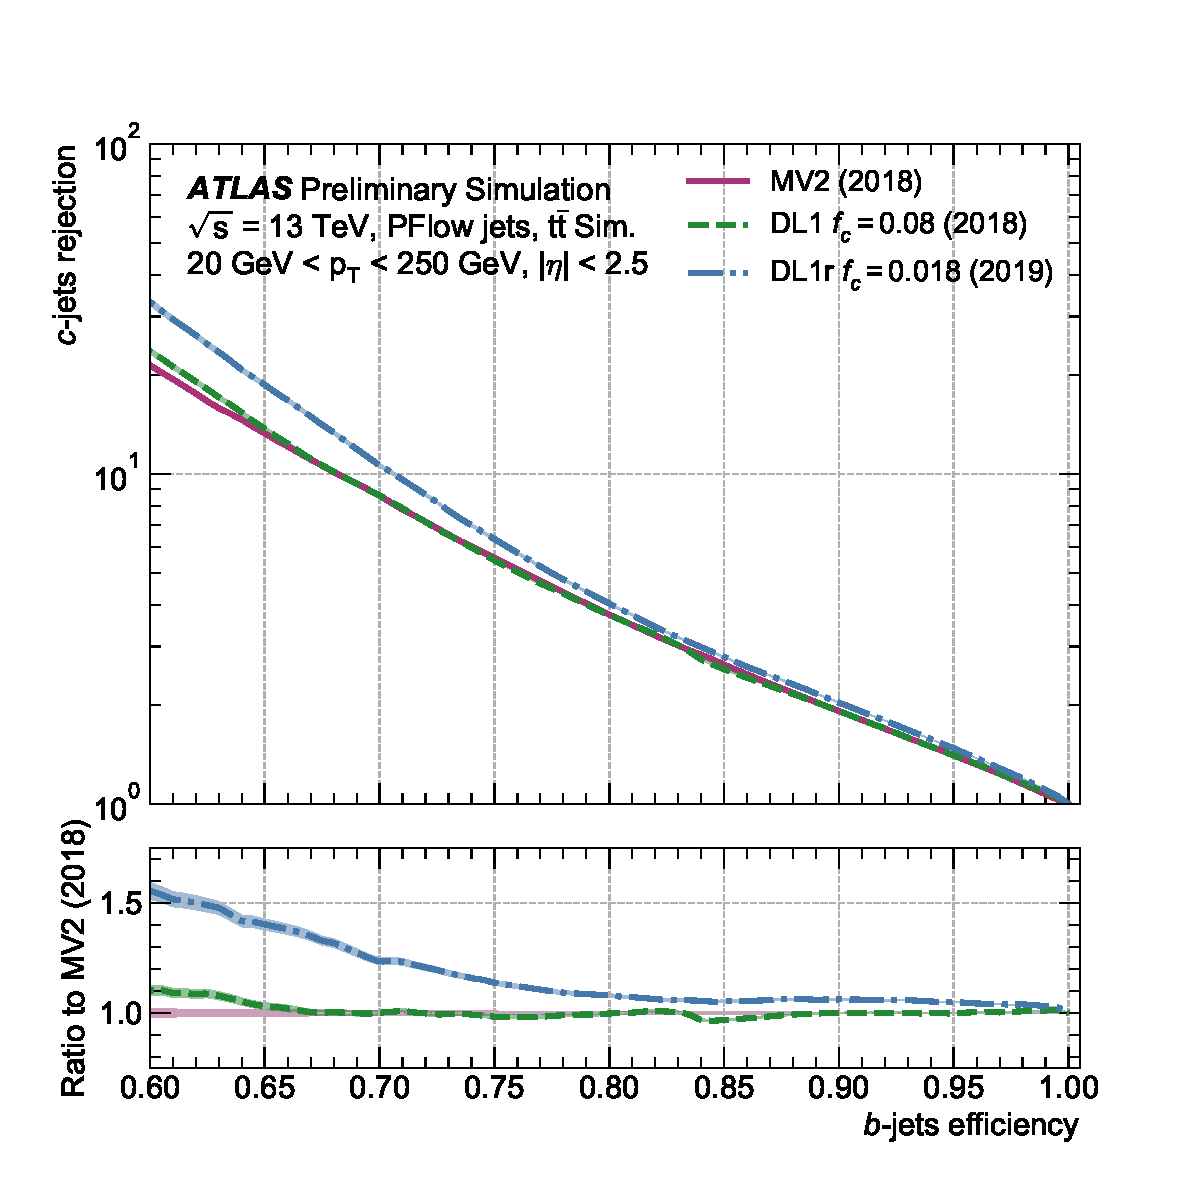
\includegraphics[width=0.48\linewidth]{\figpath/fig_01b}
    } 
    \caption{}
    \label{fig:\jetdef-fig1}
\end{figure}

\begin{figure}[htbp]
    \centering
    % light
    \subfloat[]{ 
            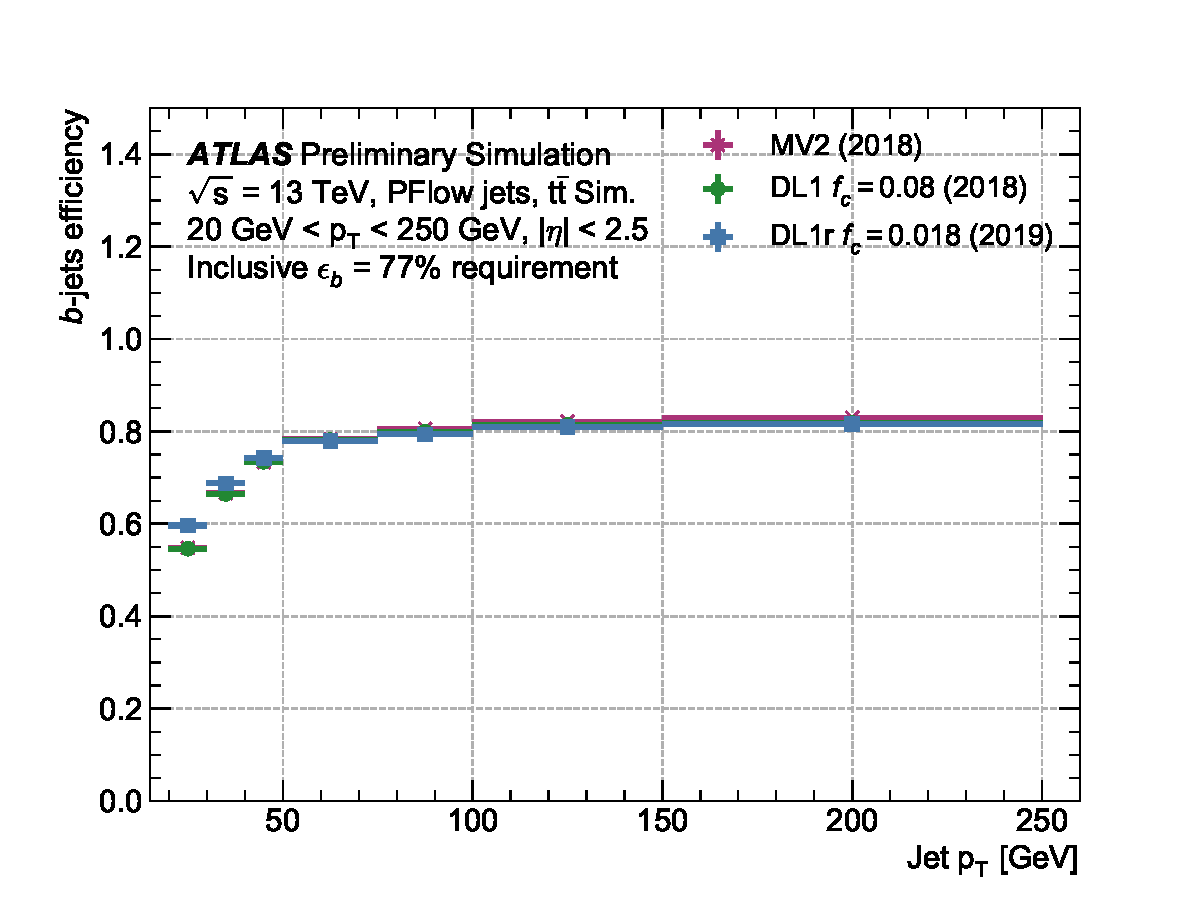
\includegraphics[width=0.33\linewidth]{\figpath/fig_02a}
    } 
     \subfloat[]{ 
            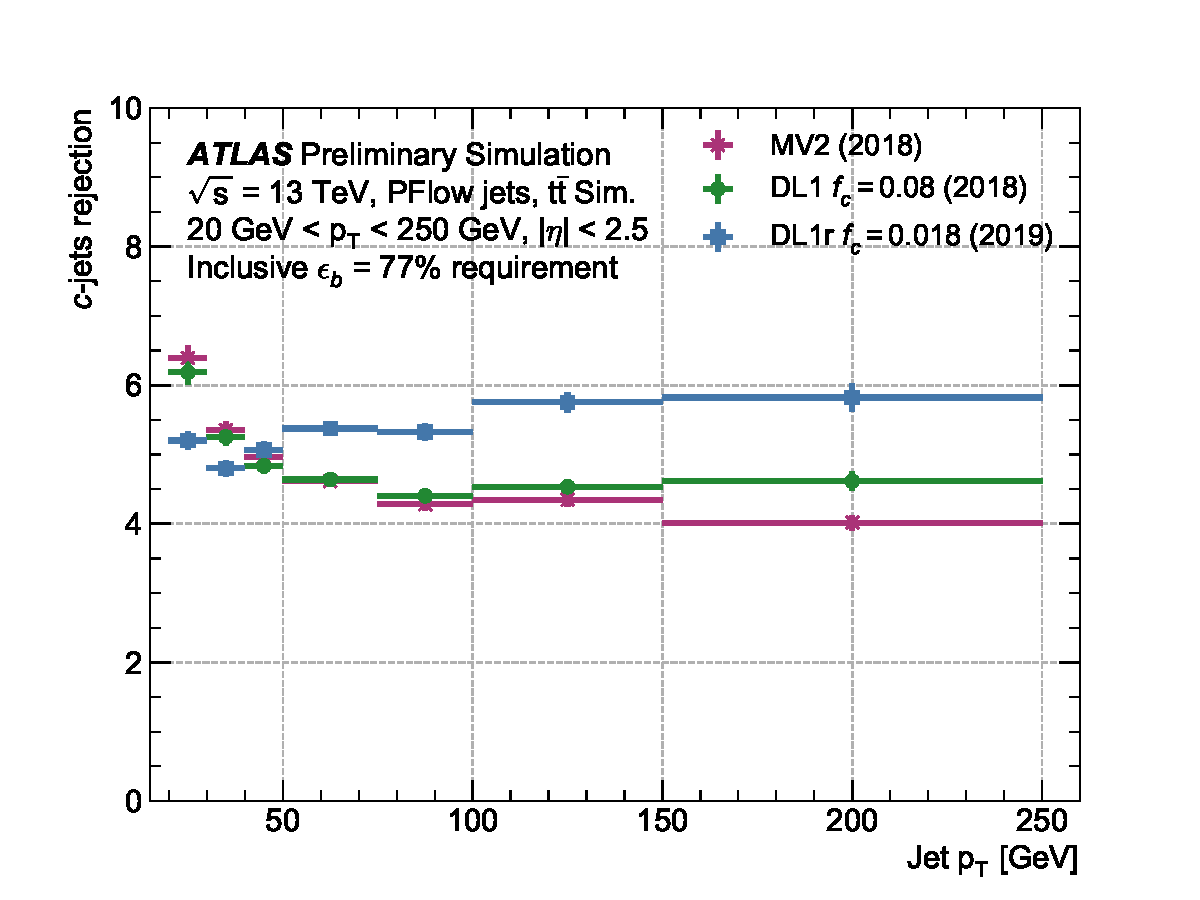
\includegraphics[width=0.33\linewidth]{\figpath/fig_02b}
    } 
    \subfloat[]{ 
            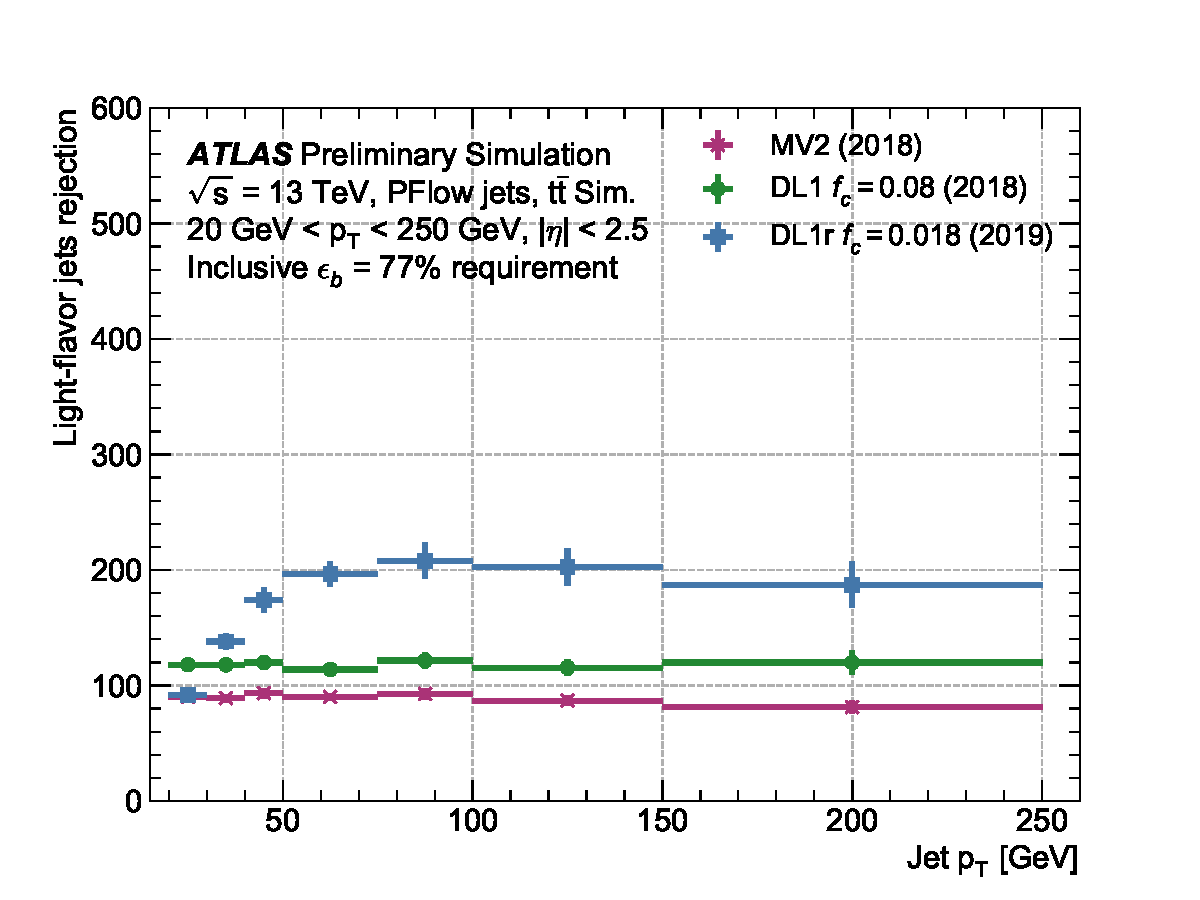
\includegraphics[width=0.33\linewidth]{\figpath/fig_02c}
    } 
    \caption{}
    \label{fig:\jetdef-fig2}
\end{figure}

\begin{figure}[htbp]
    \centering
    % light
    \subfloat[]{ 
            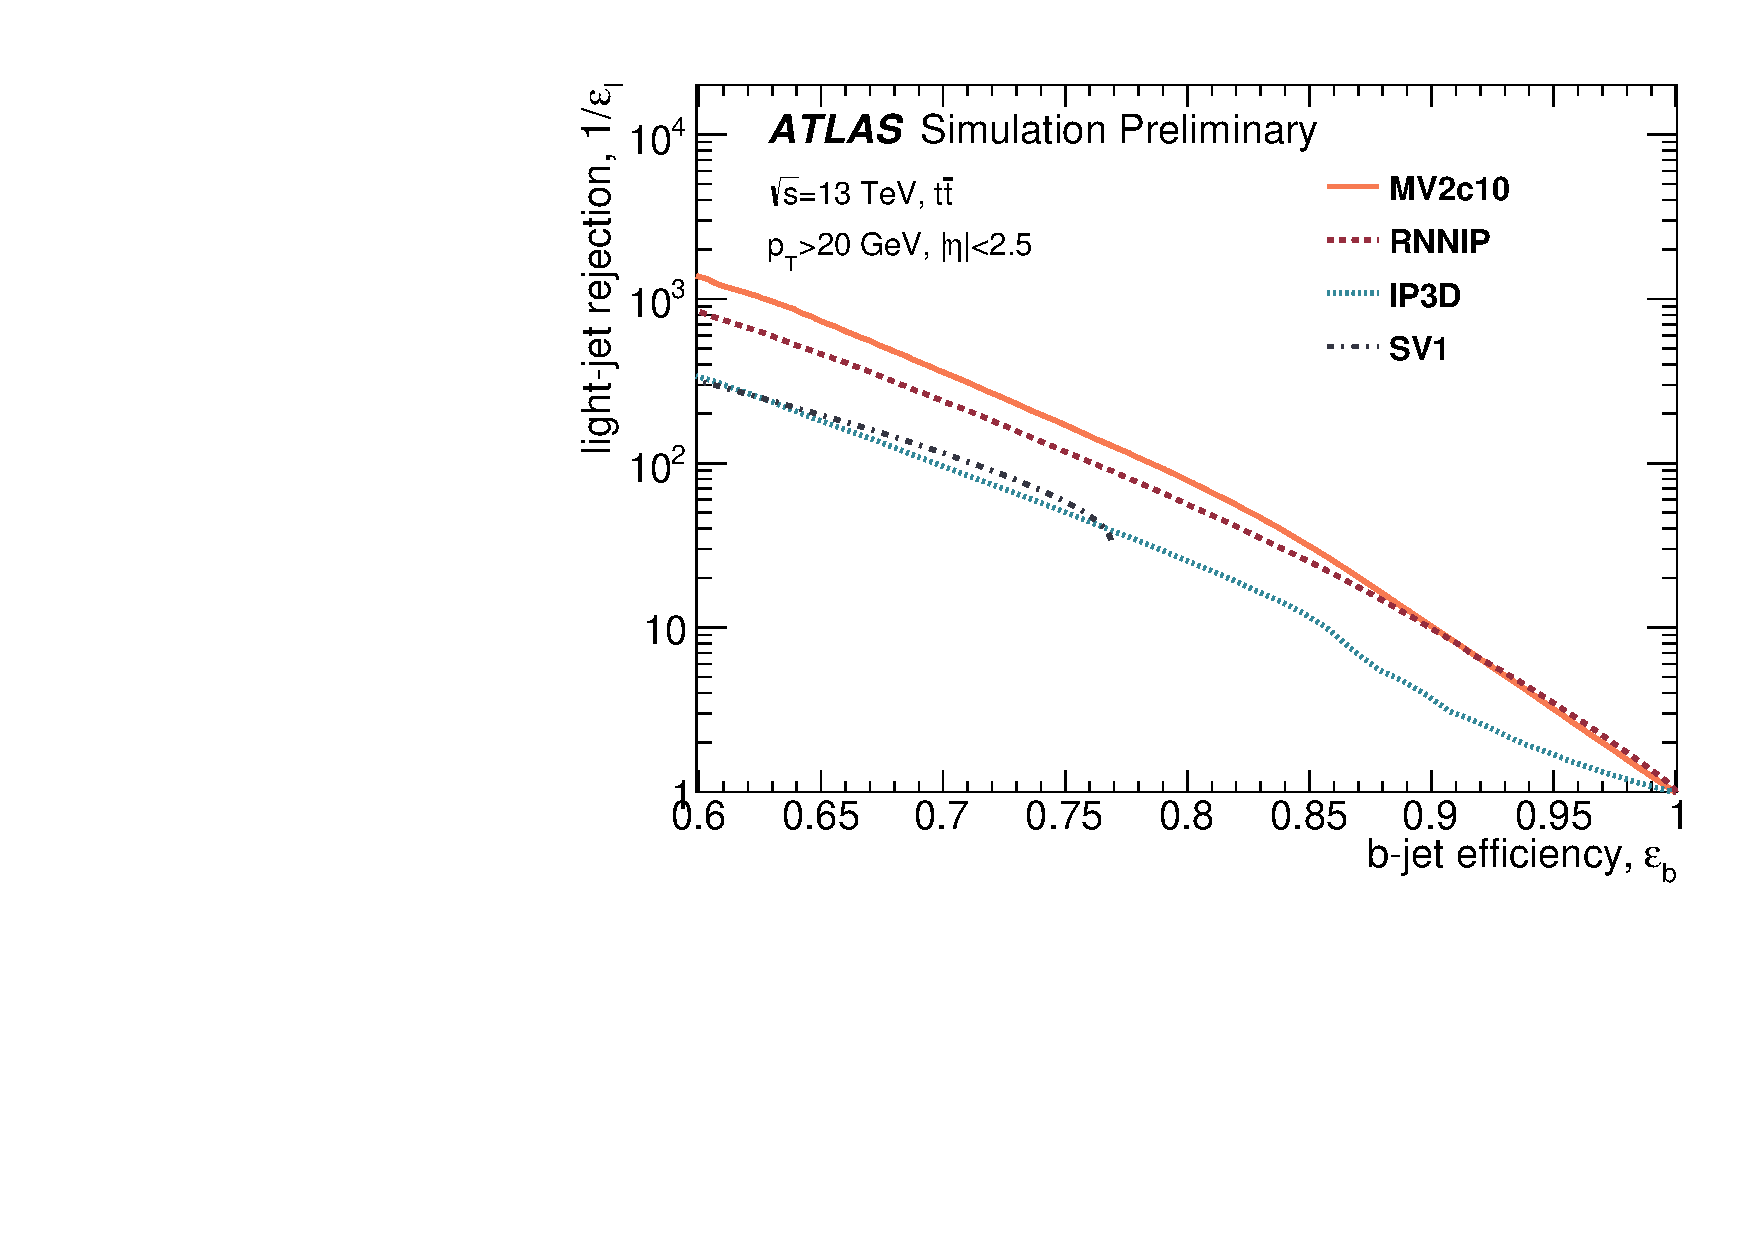
\includegraphics[width=0.48\linewidth]{\figpath/fig_03a}
    } 
     \subfloat[]{ 
            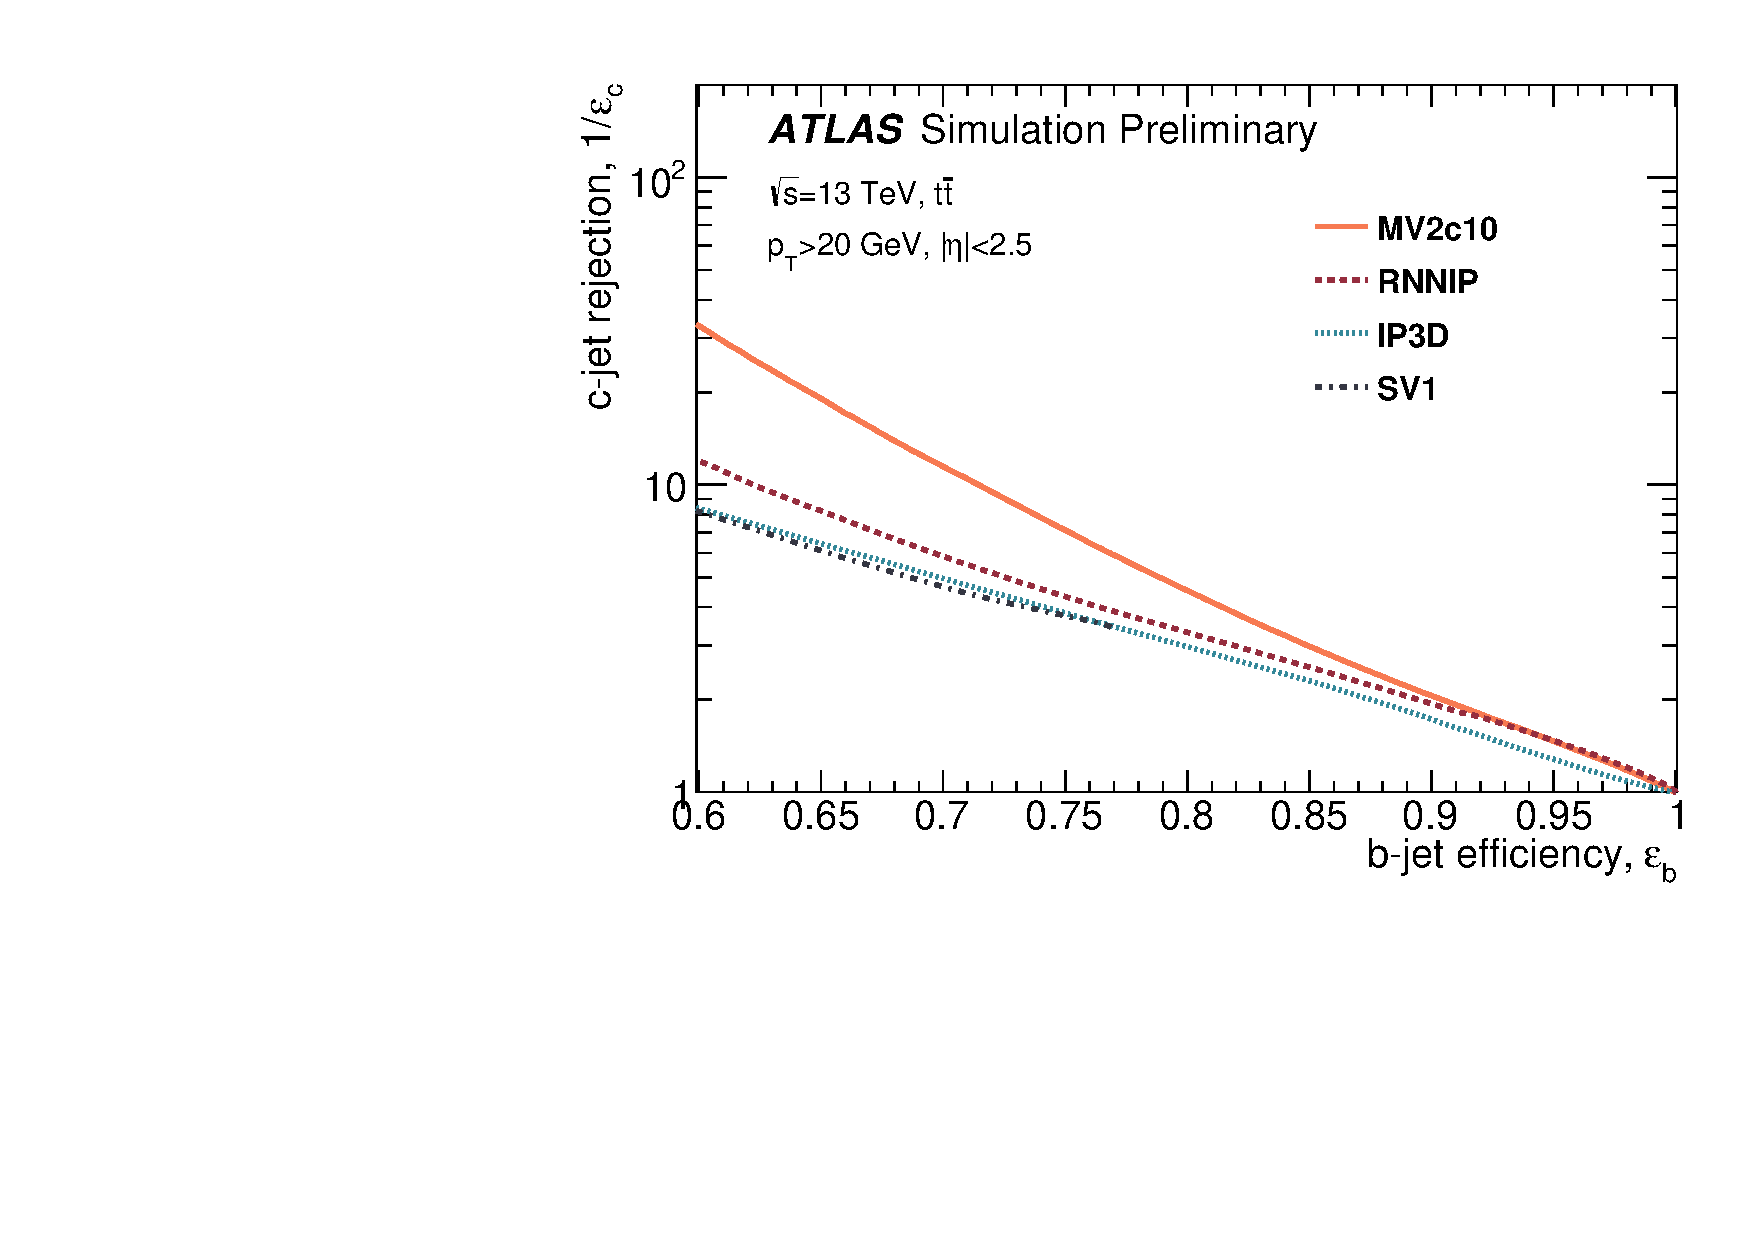
\includegraphics[width=0.48\linewidth]{\figpath/fig_03b}
    } 
    \caption{}
    \label{fig:\jetdef-fig3}
\end{figure}





%%%%%%%%%%%%%%%%%%%%%%%%%%%%%%
% VR track jets
%%%%%%%%%%%%%%%%%%%%%%%%%%%%%%

\FloatBarrier
\clearpage
\subsection{VR track jets optimization}

\begin{figure}[htbp]
  \centering
  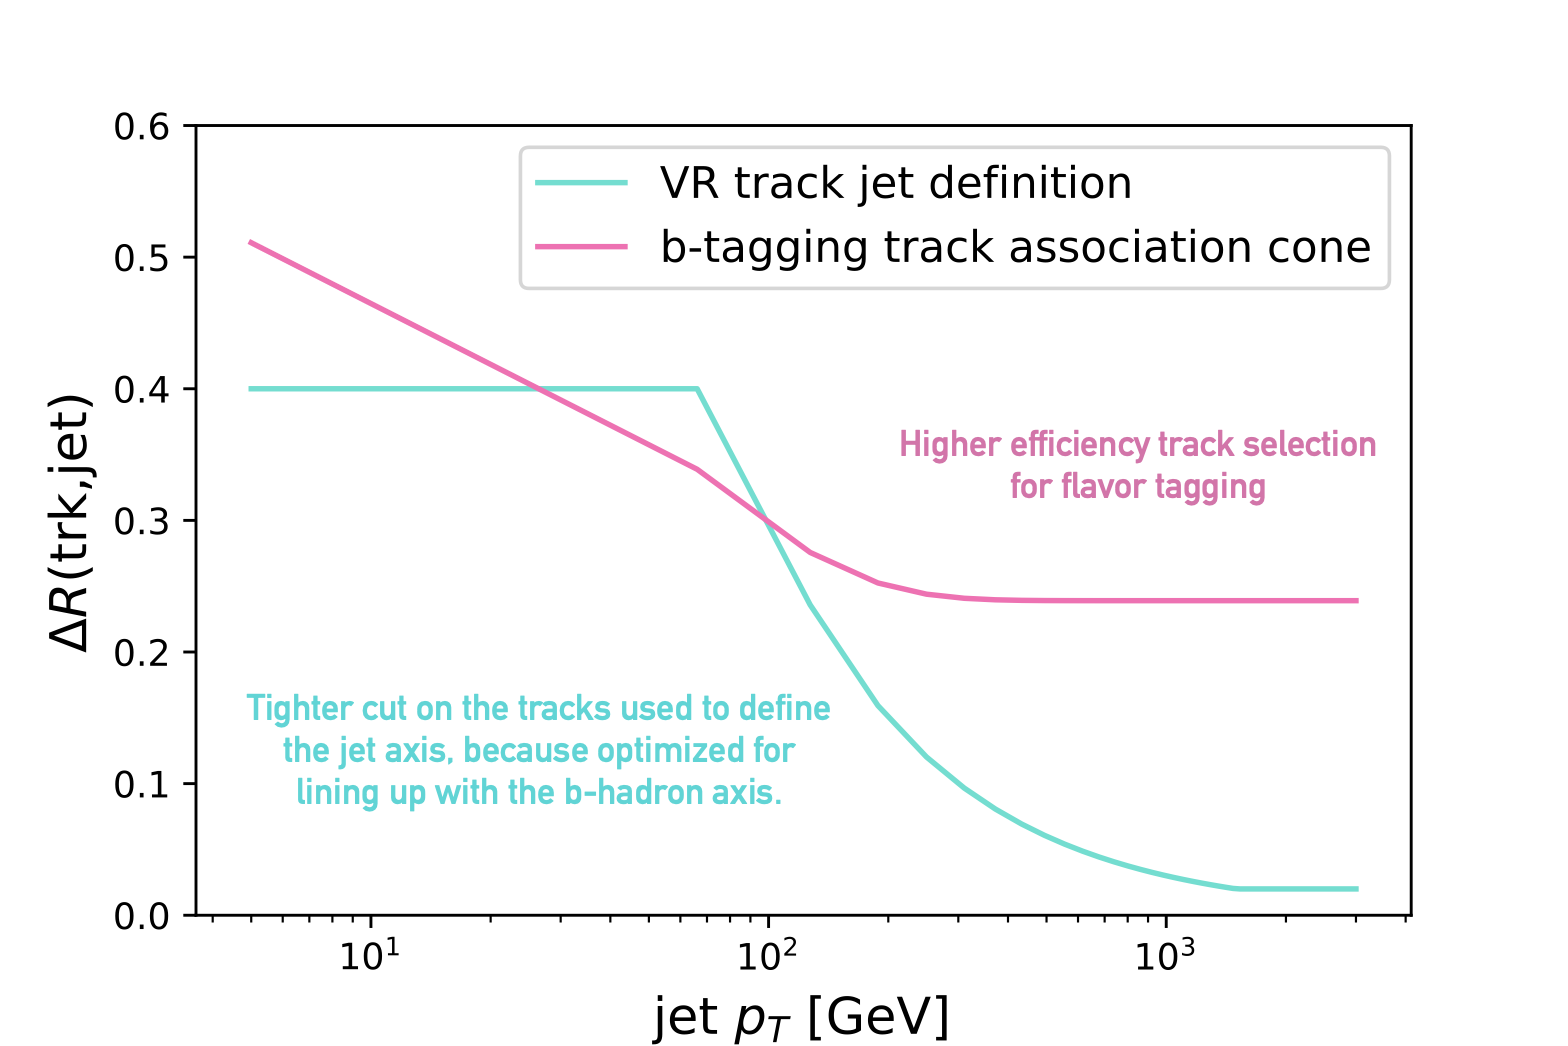
\includegraphics[width=.6\textwidth]{figures/ftag/VR trainings/vr-ftag-dR-cuts}
  \caption{Comparison of the $\Delta R$ track cuts that (1) define the jet axis for the VR track jet (cyan) and (2) the tracks used as input to the FTAG algorithms (pink).}
  \label{fig:pt-VR-pflow}
\end{figure}



\hl{I had to have had a dR matching in this plot \ldots let's look up what it was!}

\begin{figure}[htbp]
  \centering
  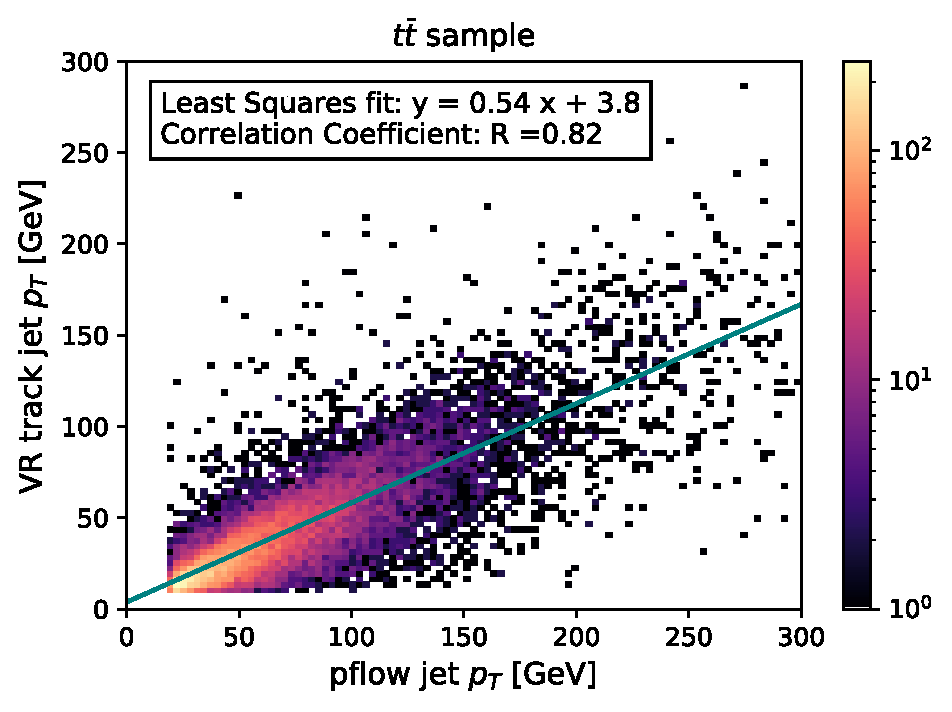
\includegraphics[width=.45\textwidth]{figures/ftag/VR trainings/pt-VR-pflow-ttvar}
  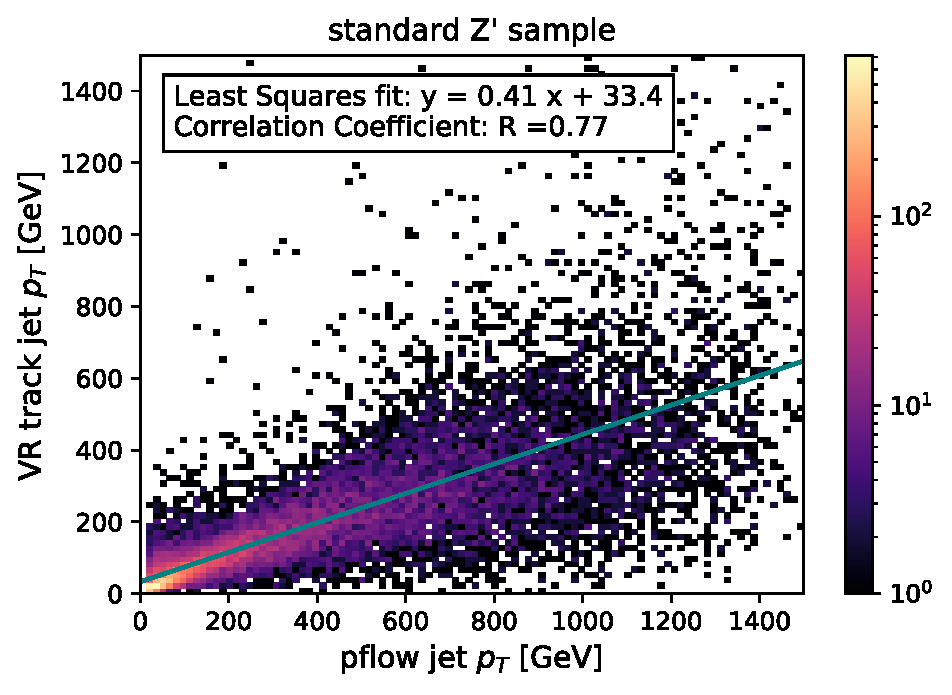
\includegraphics[width=.45\textwidth]{figures/ftag/VR trainings/pt-VR-pflow-std-Zprime}
  \caption{Comparison of the PFlow and VR track jet \pt for jet reconstruction.}
  \label{fig:pt-VR-pflow}
\end{figure}

Note: This plot \emph{motivated} us to move the pT cut on the light and c-jets to 125~GeV (although we kept the b-hadron \pt cut at 250 GeV).

\begin{figure}[htbp]
  \centering
  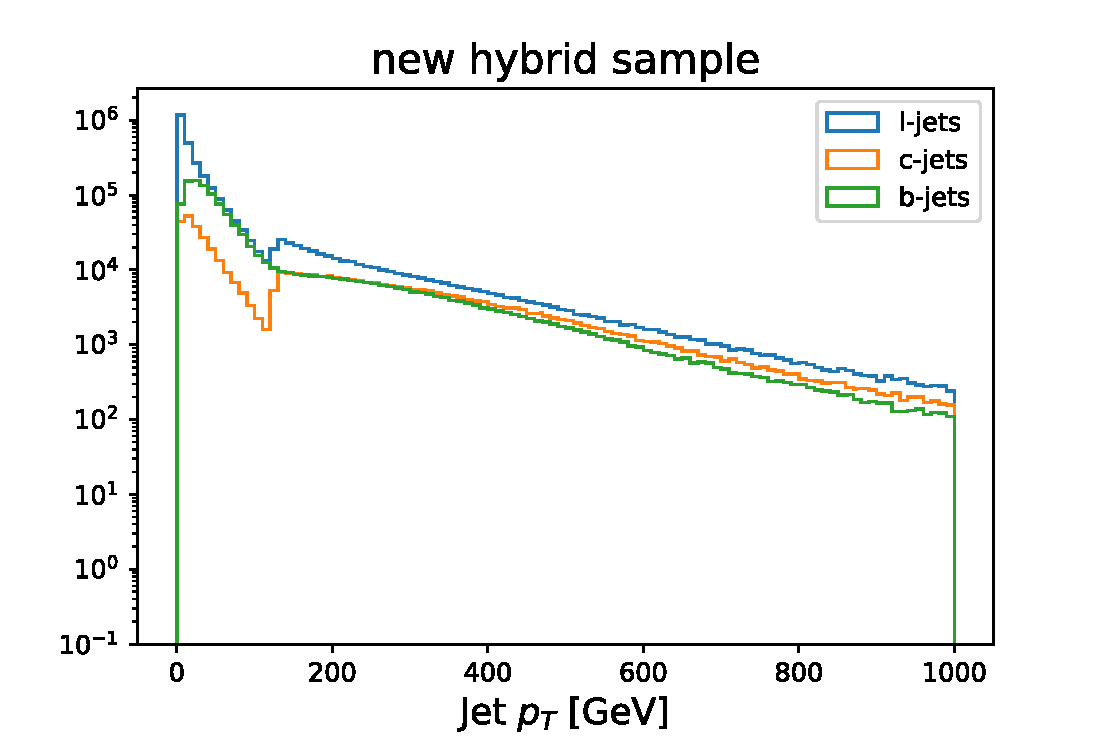
\includegraphics[width=.6\textwidth]{figures/ftag/VR trainings/pt-hyb-vr}
  \caption{The \pt spectrum for the VR track jets using the modified sample cut of 125~GeV for the light jet and \Pqb-jet \pt.}
  \label{fig:pflow-pt-extended-hybrid}
\end{figure}



\begin{figure}
\centering
\subfloat[light rejection]{
	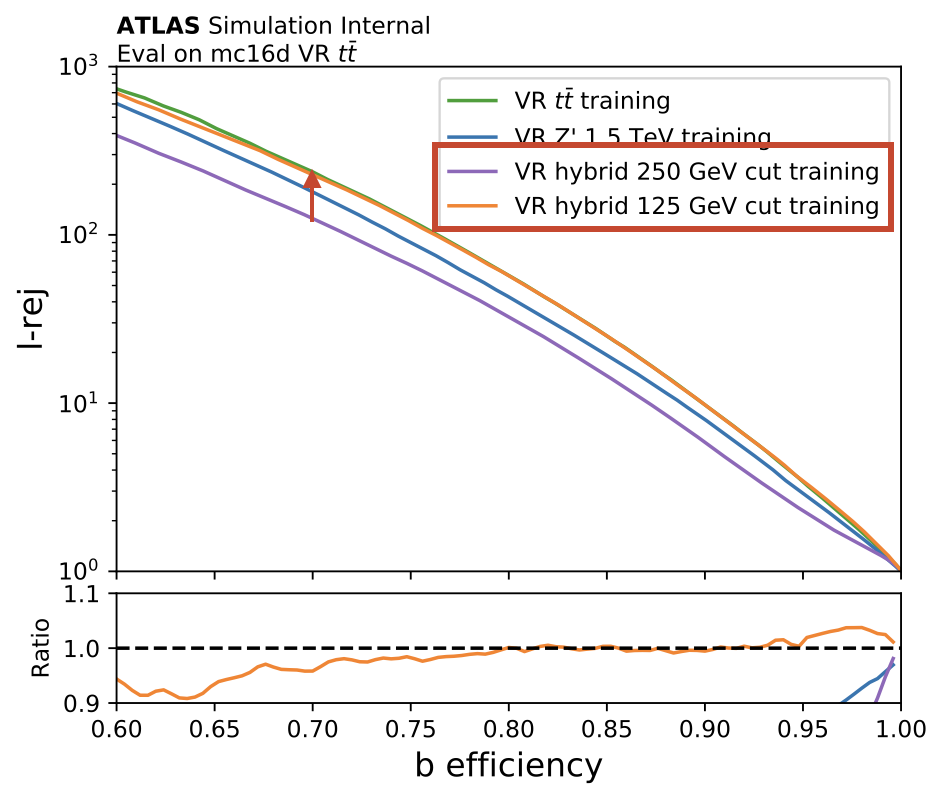
\includegraphics[width=0.45\textwidth]{{figures/ftag/VR\ Trainings/roc-new-cut-l-ttbar}}
	}
\subfloat[\Pqc rejection]{
	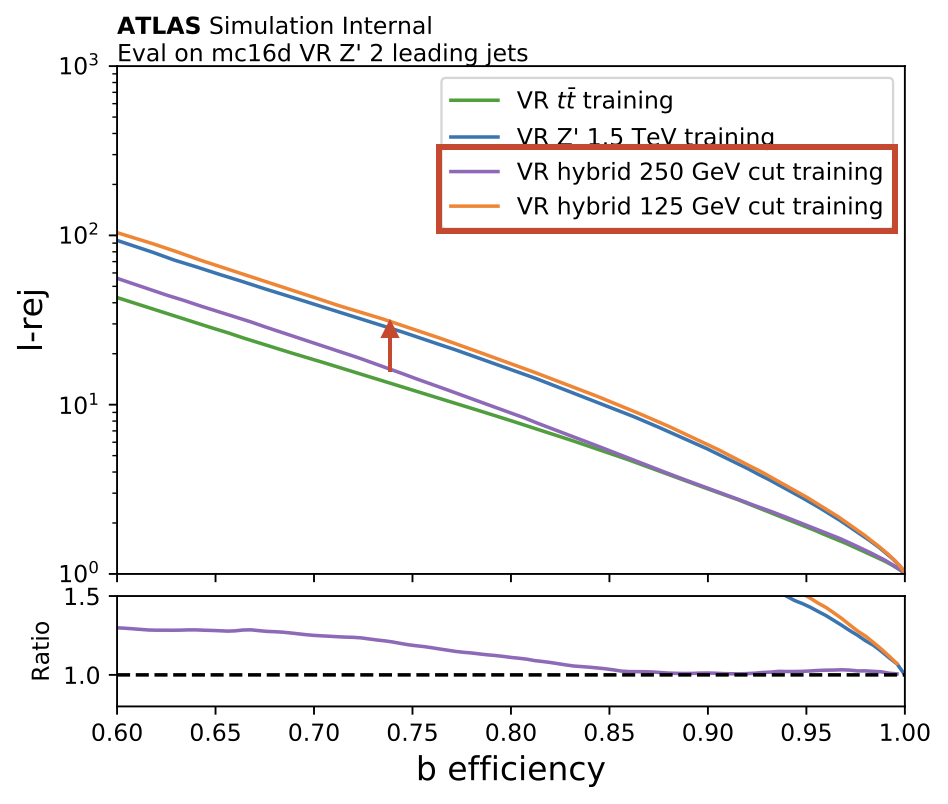
\includegraphics[width=0.45\textwidth]{{figures/ftag/VR\ Trainings/roc-new-cut-l-Zprime}}
	}
\caption{}
\label{fig:VR-improvements}
\end{figure}



\begin{figure}
\centering
\subfloat[light rejection]{
	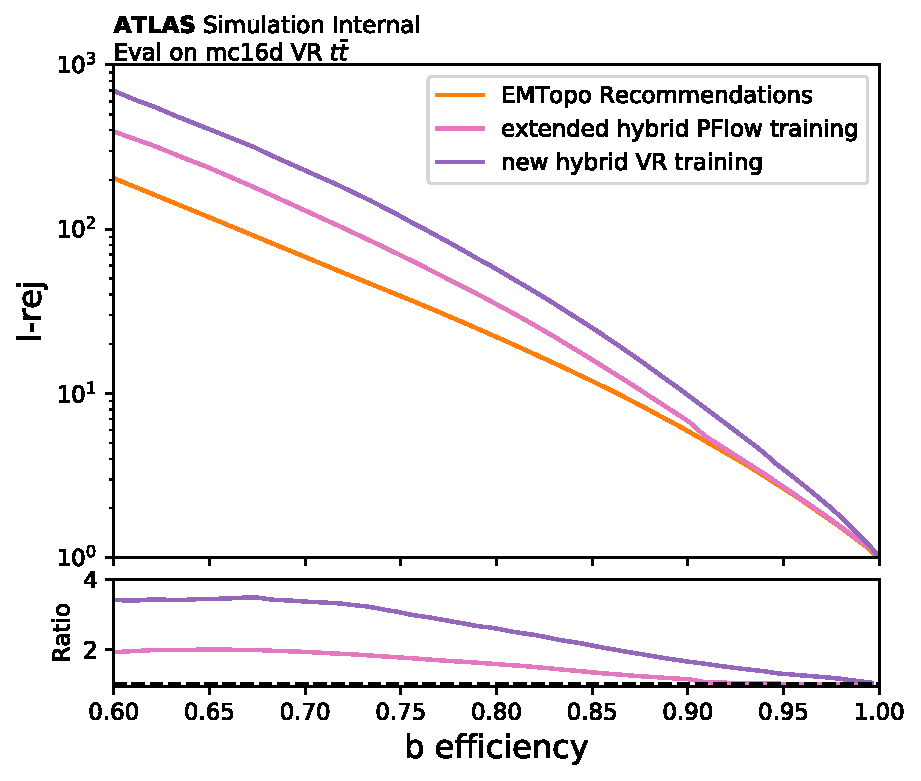
\includegraphics[width=0.45\textwidth]{{figures/ftag/VR\ Trainings/roc-vr-trainings-l}}
	}
\subfloat[\Pqc rejection]{
	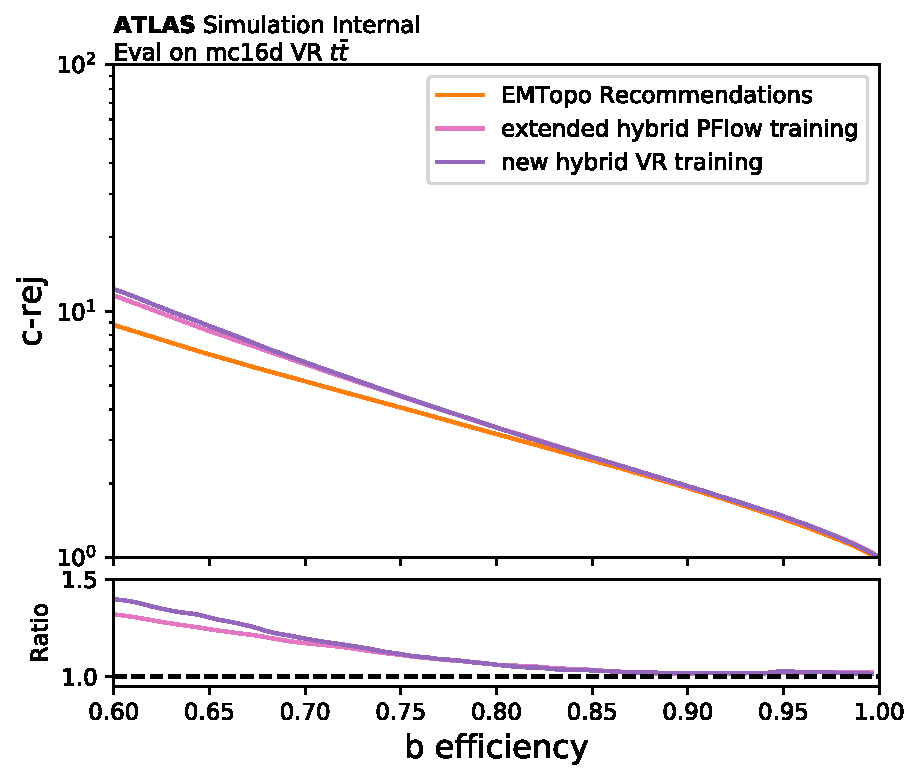
\includegraphics[width=0.45\textwidth]{{figures/ftag/VR\ Trainings/roc-vr-trainings-c}}
	}
\caption{}
\label{fig:VR-improvements}
\end{figure}

\begin{enumerate}
	\item \textcolor{orange}{EMTopo Rec: What we were applying to VR track jets now}
	\item \textcolor{deeppink}{Ext Pflow: If we applied the my new pflow training to VR track jets}
	\item \textcolor{mediumpurple}{New hybrid VR training: NEW dedicated VR training}
\end{enumerate}




\def\jetdef{VR}
% http://atlas.web.cern.ch/Atlas/GROUPS/PHYSICS/PLOTS/FTAG-2019-006/

\def\figpath{figures/ftag/\jetdef \ trainings}

\begin{figure}[htbp]
    \centering
    % light
    \subfloat[]{ 
            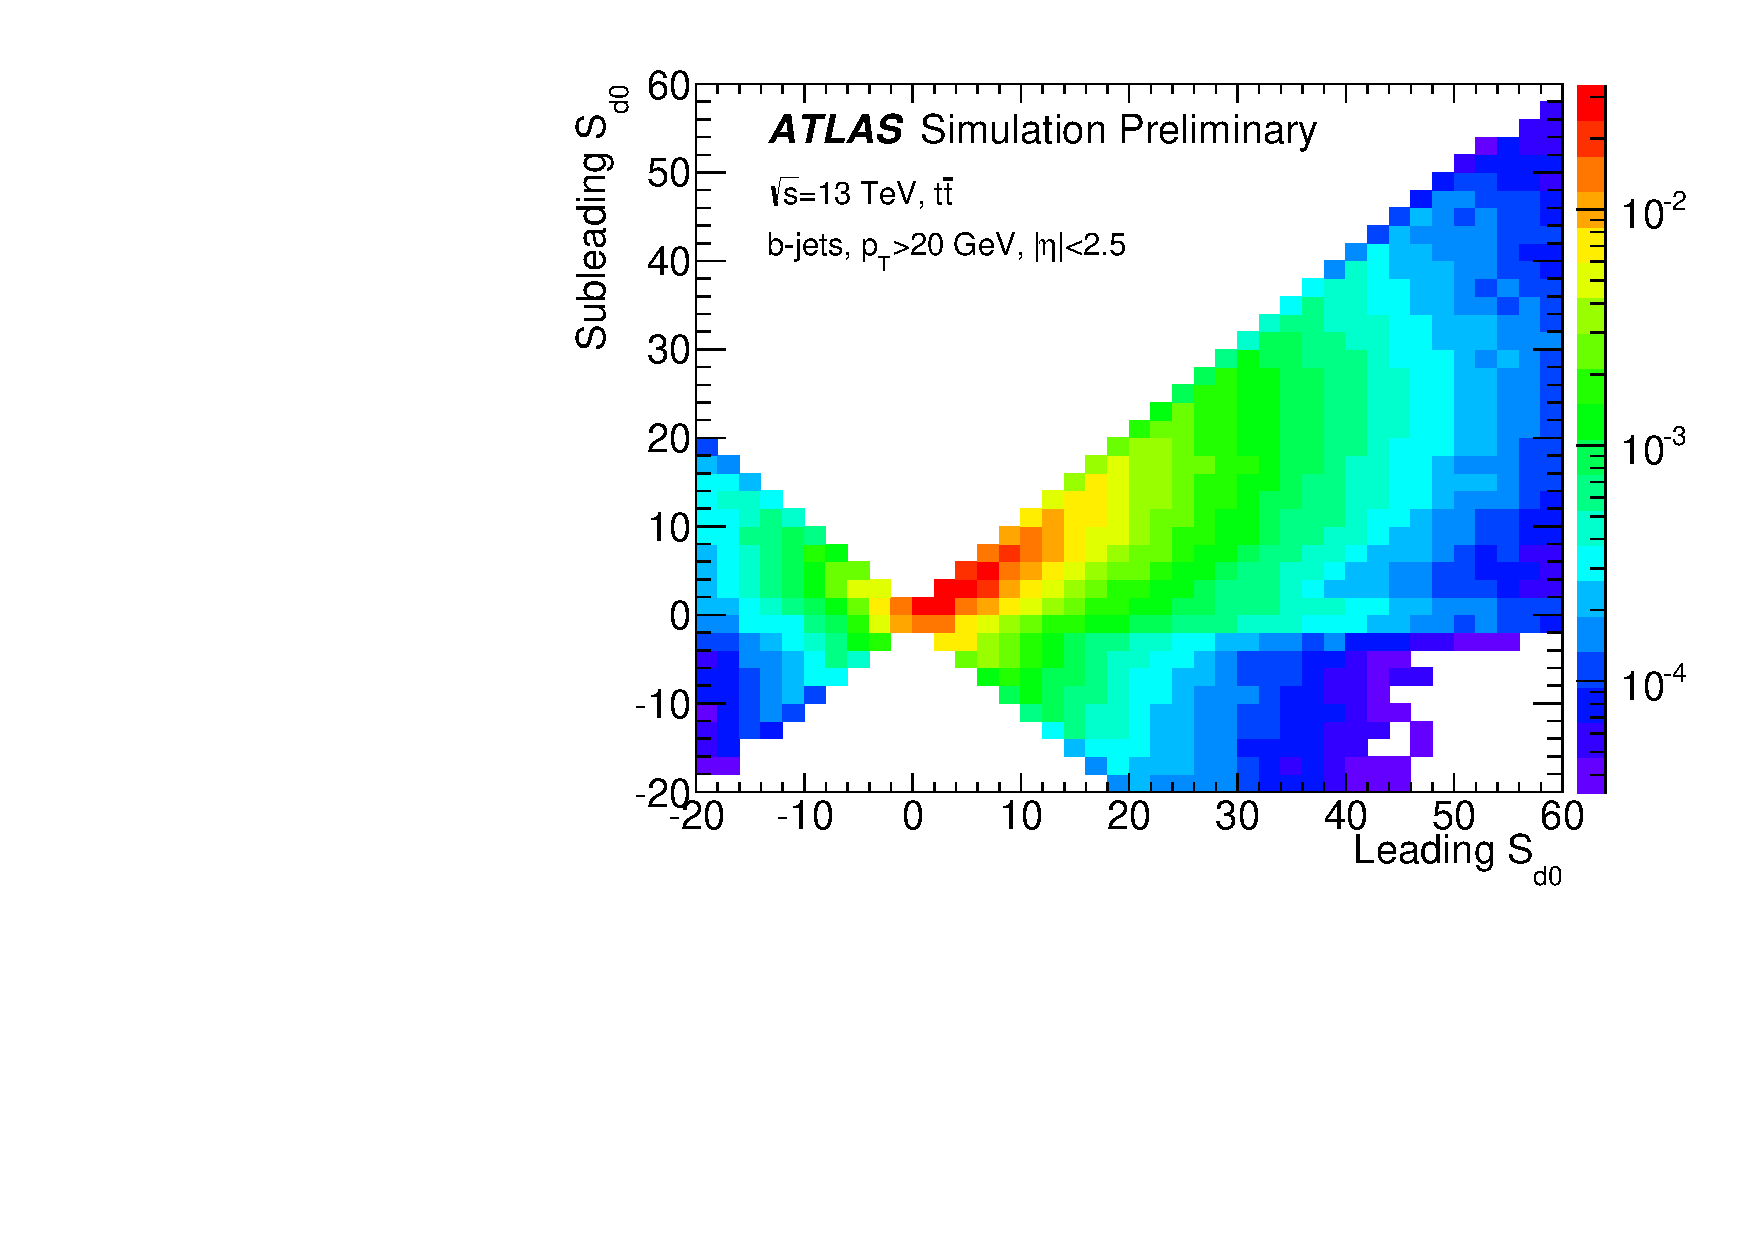
\includegraphics[width=0.48\linewidth]{\figpath/fig_01a}
    } 
     \subfloat[]{ 
            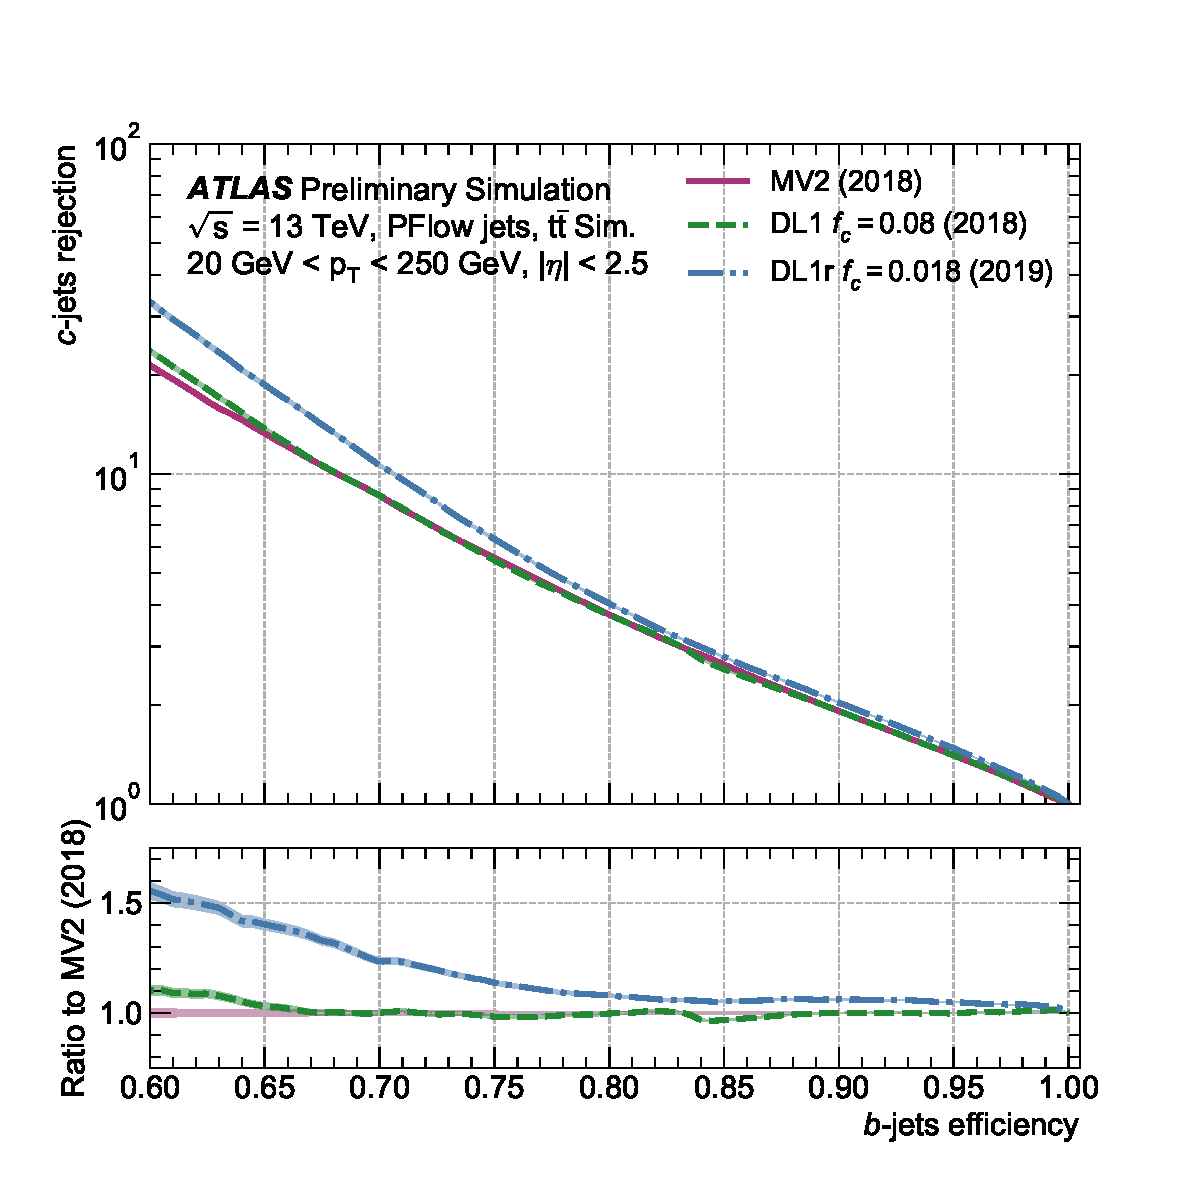
\includegraphics[width=0.48\linewidth]{\figpath/fig_01b}
    } 
    \caption{}
    \label{fig:\jetdef-fig1}
\end{figure}

\begin{figure}[htbp]
    \centering
    % light
    \subfloat[]{ 
            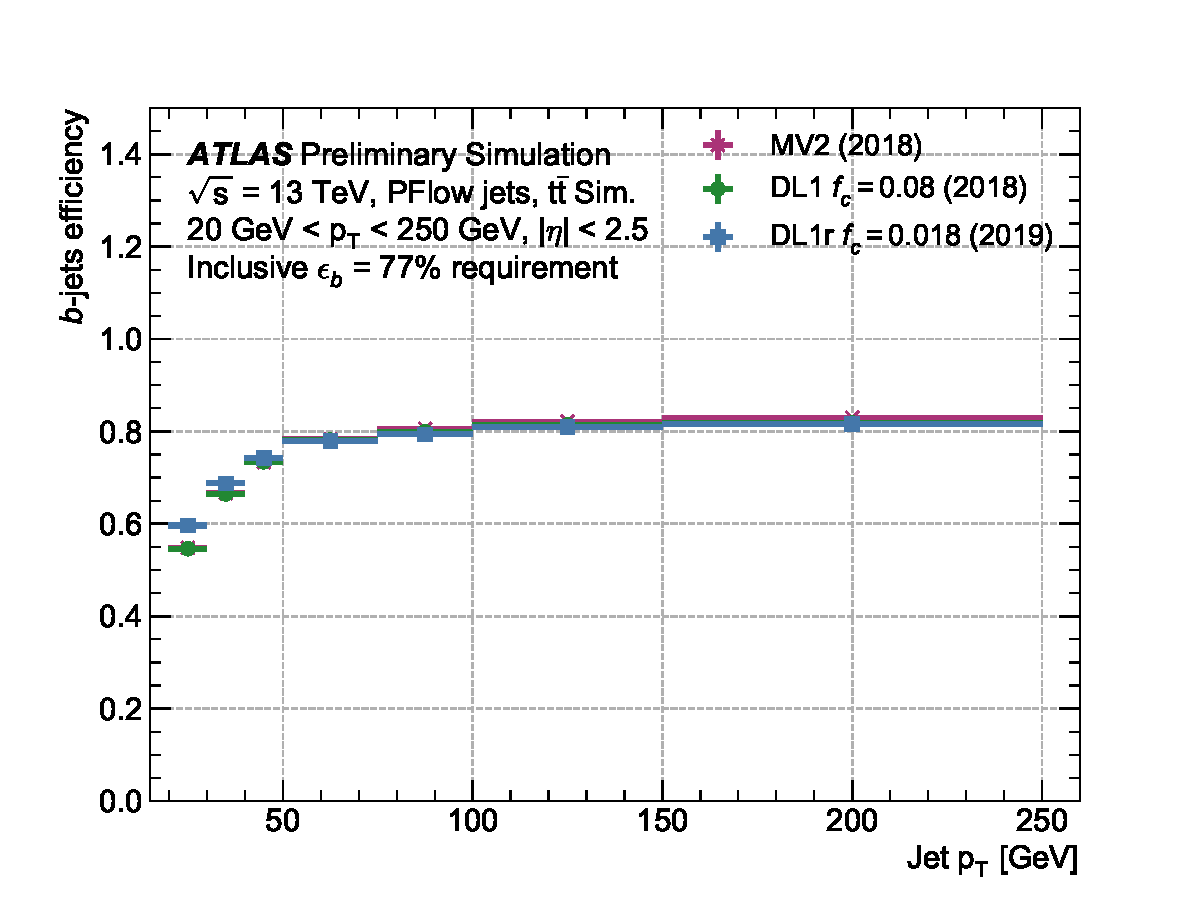
\includegraphics[width=0.33\linewidth]{\figpath/fig_02a}
    } 
     \subfloat[]{ 
            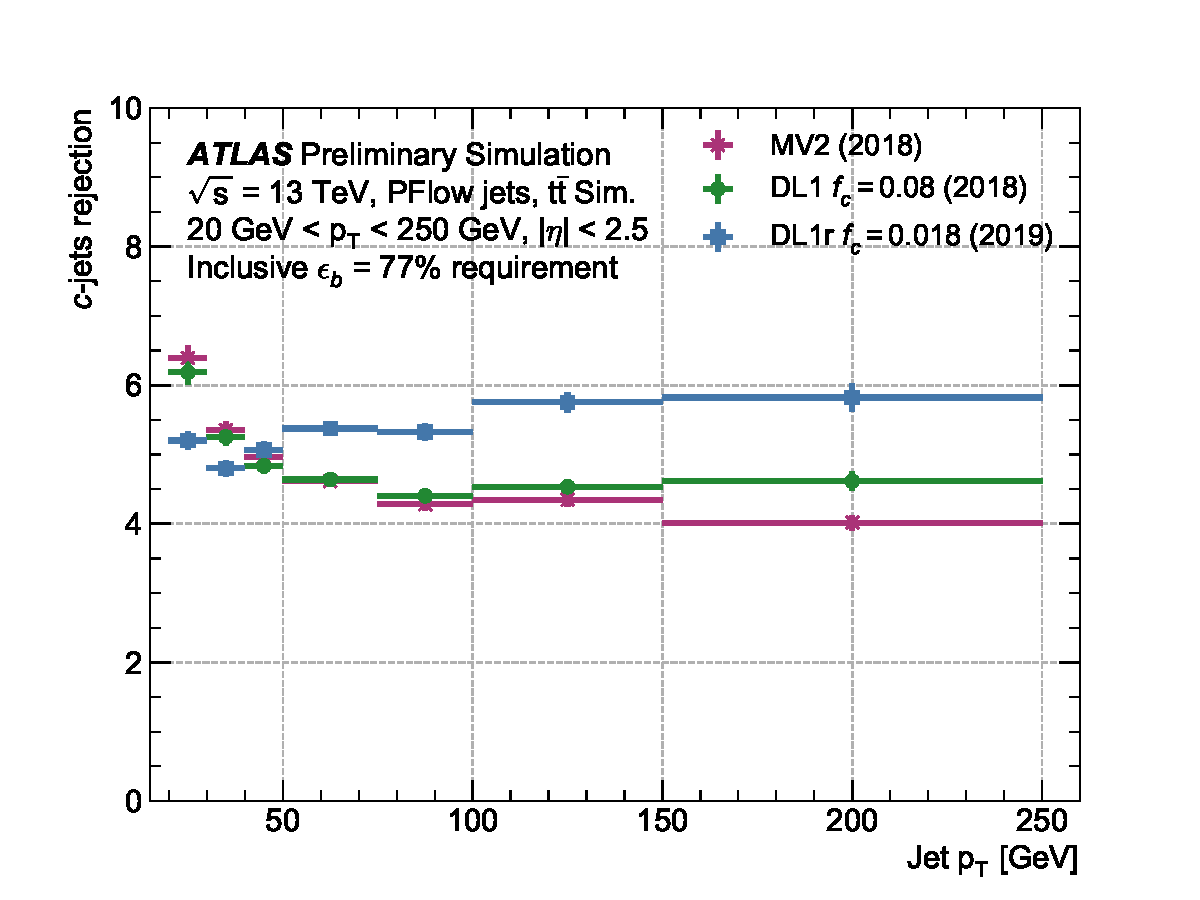
\includegraphics[width=0.33\linewidth]{\figpath/fig_02b}
    } 
    \subfloat[]{ 
            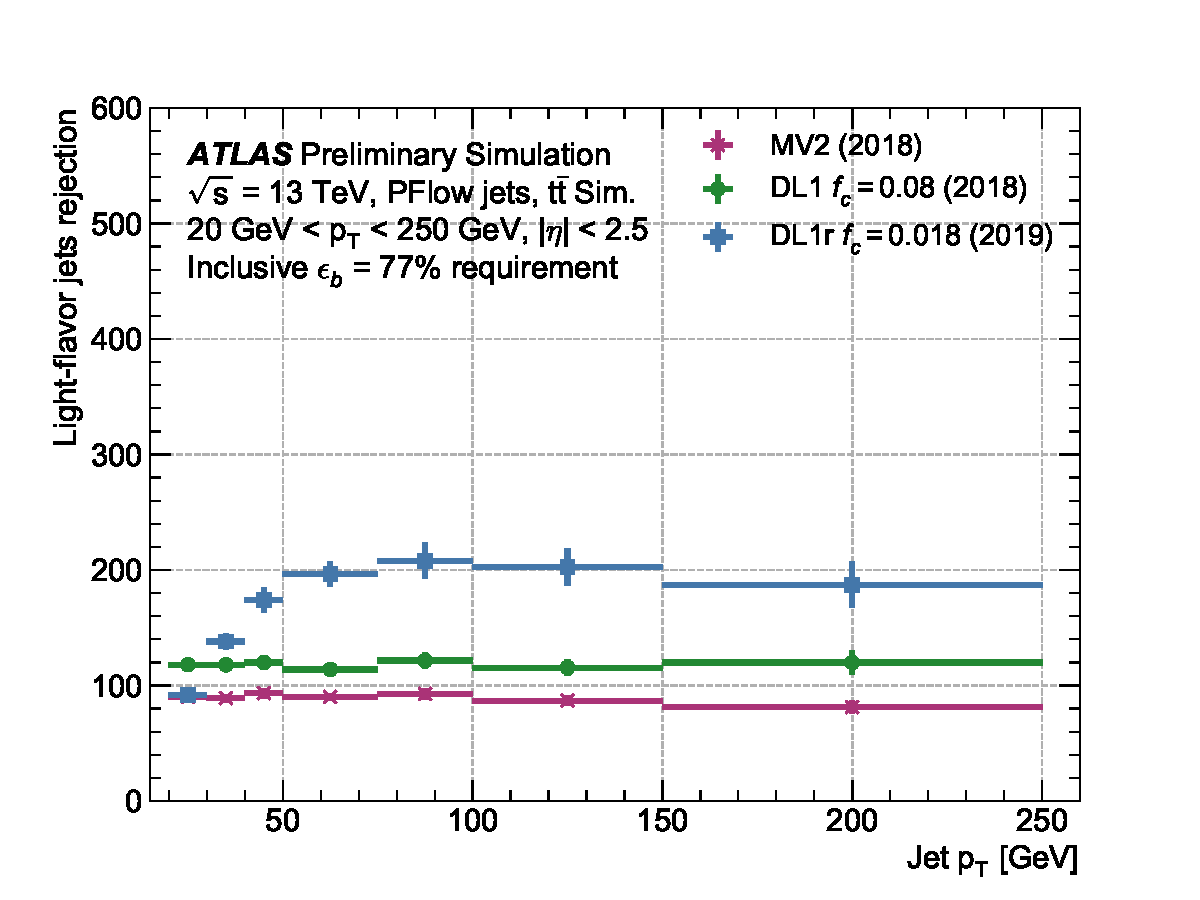
\includegraphics[width=0.33\linewidth]{\figpath/fig_02c}
    } 
    \caption{}
    \label{fig:\jetdef-fig2}
\end{figure}

\begin{figure}[htbp]
    \centering
    % light
    \subfloat[]{ 
            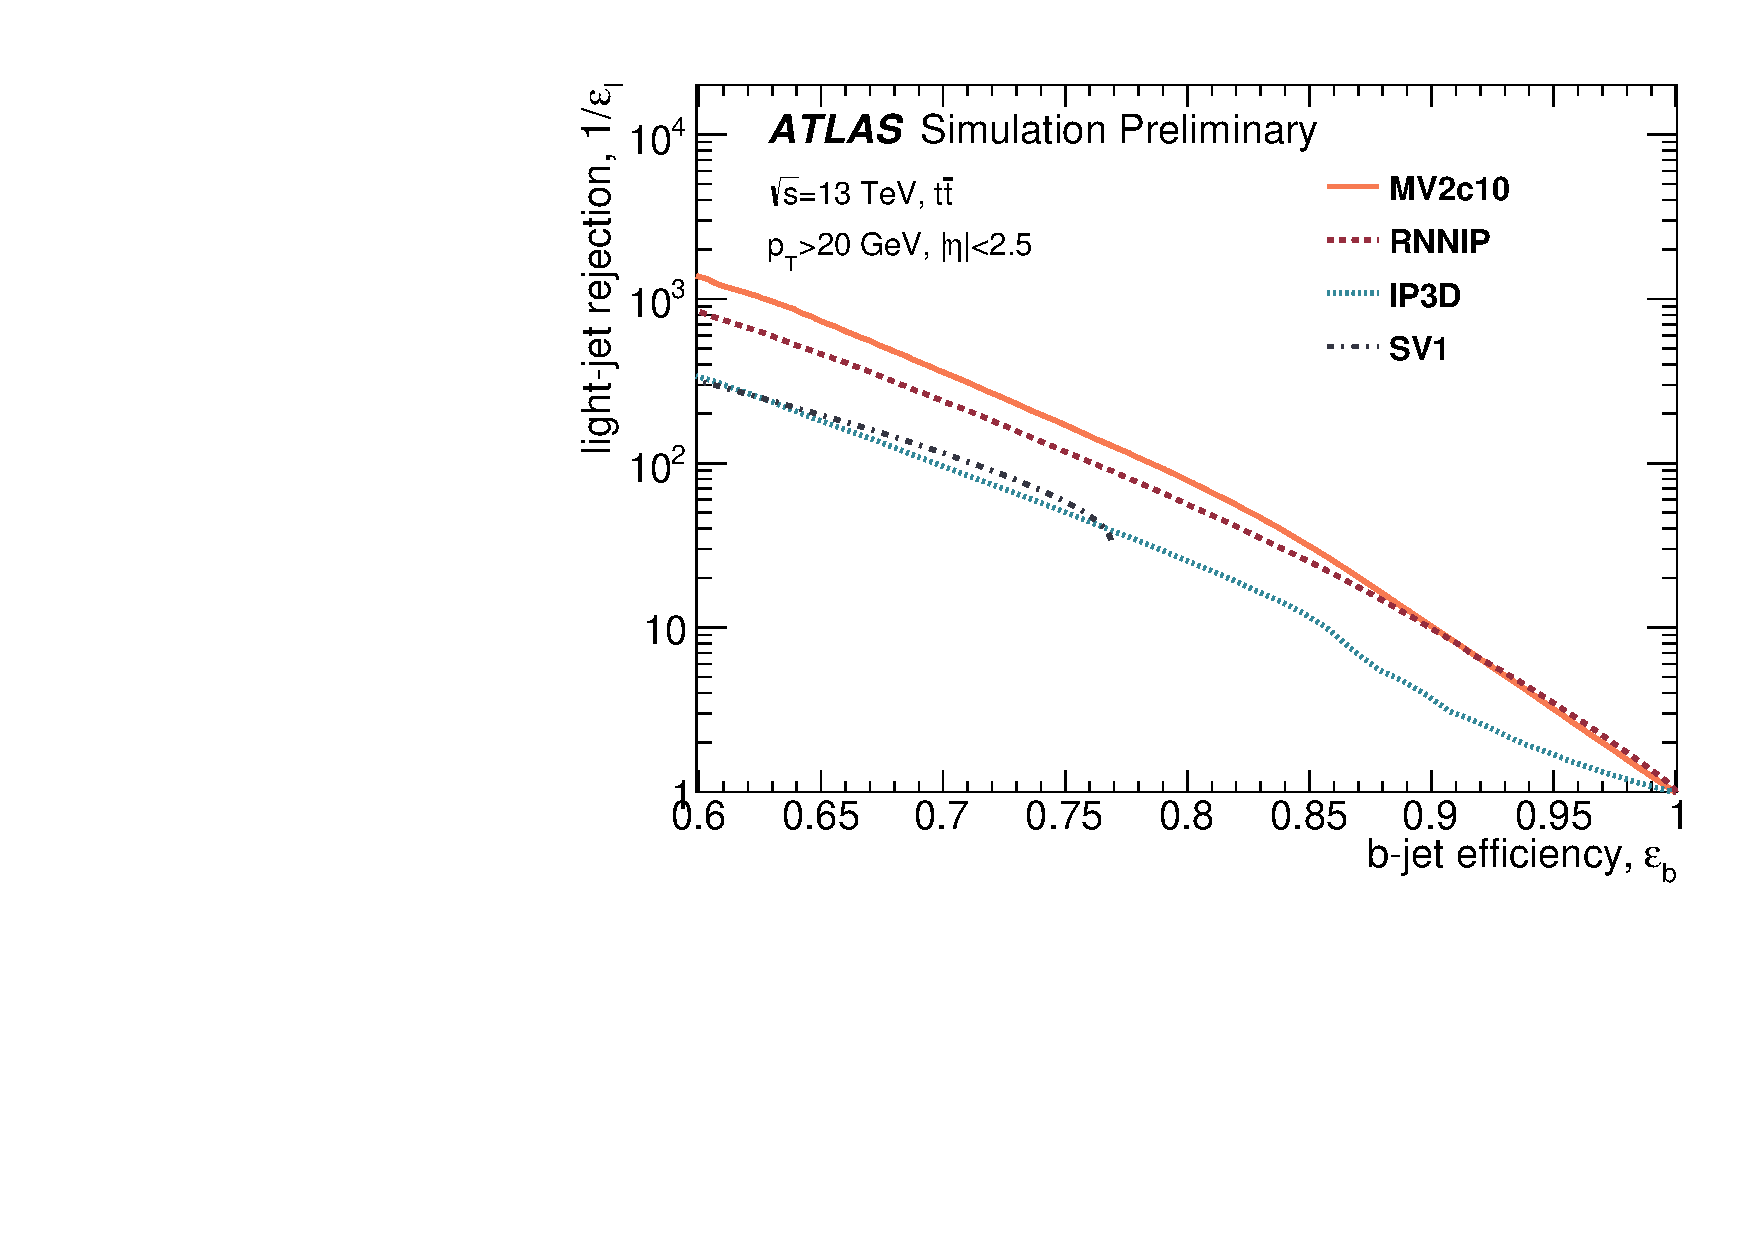
\includegraphics[width=0.48\linewidth]{\figpath/fig_03a}
    } 
     \subfloat[]{ 
            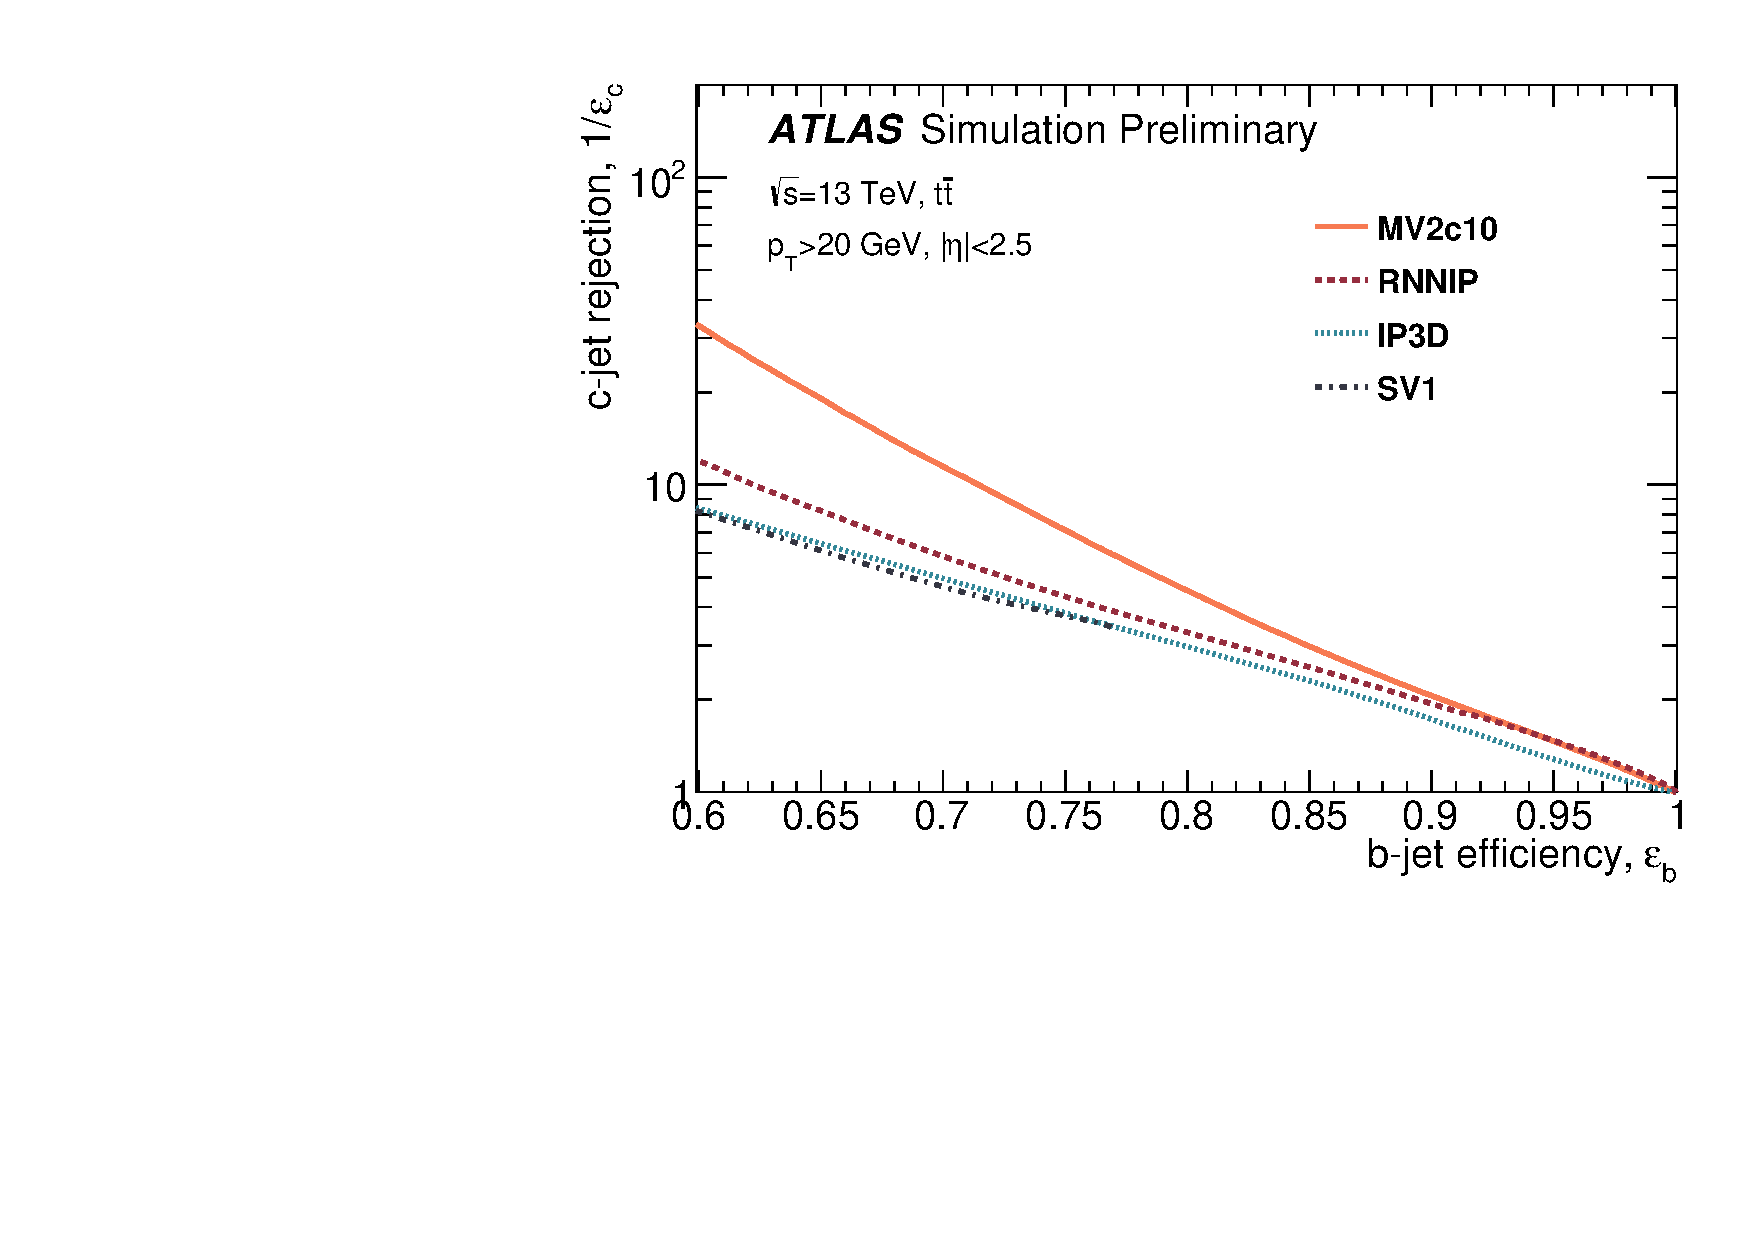
\includegraphics[width=0.48\linewidth]{\figpath/fig_03b}
    } 
    \caption{}
    \label{fig:\jetdef-fig3}
\end{figure}

\subsection{Impact of FTAG improvements on analyses}

\begin{figure}
\centering
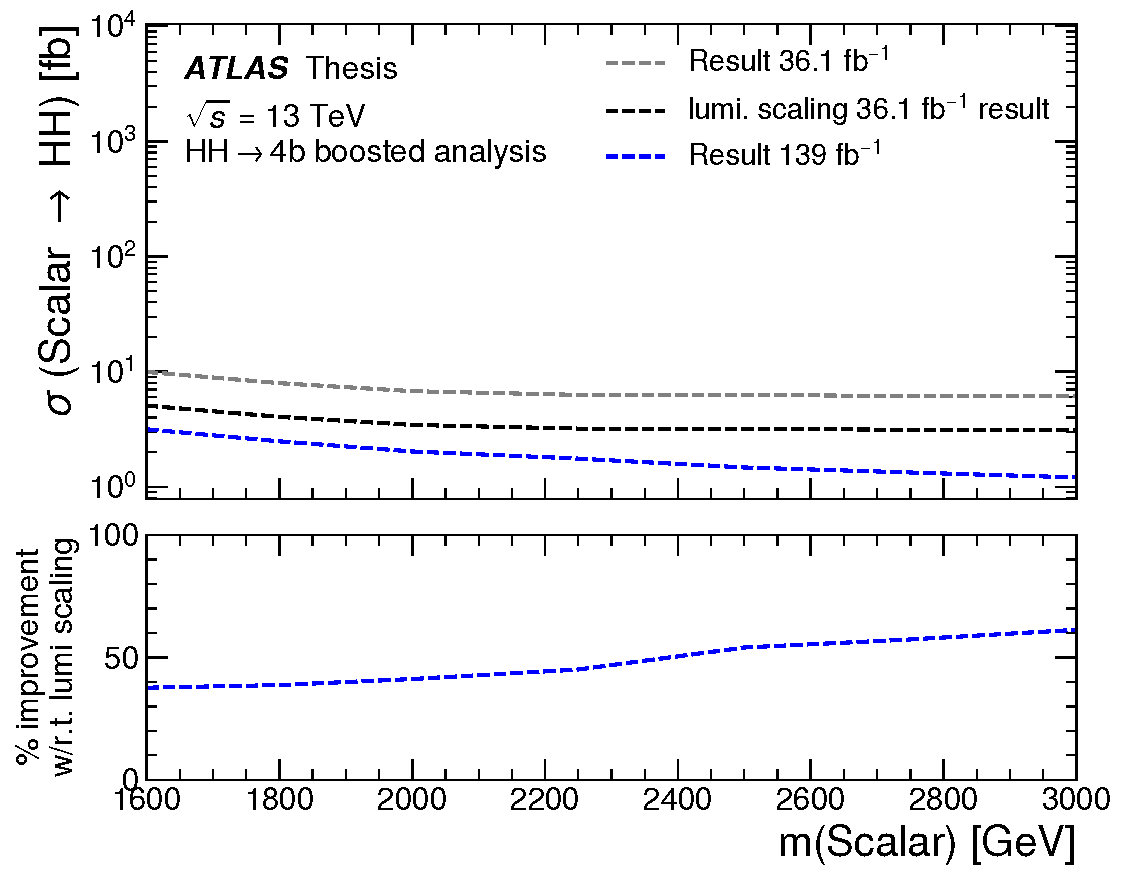
\includegraphics[width=\textwidth]{figures/my_dihiggs/HH4b-boosted-vr-trk-jet-improvements.pdf}
\caption{Need to cite the 36 ifb and 139 ifb.}
\label{fig:boosted-vr-trk-jet-improvements}
\end{figure}
